\documentclass[12pt]{article}
\usepackage[font=small,labelfont=bf]{caption}
\usepackage{graphicx}
\usepackage{amsmath}
\usepackage{hyperref}\usepackage{color}
\usepackage{parskip}
\usepackage{float}
\usepackage{tabularx}
\usepackage{appendix}
\usepackage{rotating} \usepackage{verbatim} \usepackage{lscape}
\usepackage{dcolumn} \usepackage{ctable} \usepackage{amssymb}
\usepackage{longtable}
\usepackage{threeparttable}
\usepackage{pdflscape}
\usepackage{cases}
\usepackage{geometry}


 \usepackage[style=authoryear,backend=biber, url=true, maxcitenames=2]{biblatex}
 \addbibresource{new.bib}
\title{Complementarity between Exporting, Importing and Productivity: Evidence from India}
\author{Arjun Gupta (2014592/823125)}
% \institution{Tilburg University}
\newcommand{\alert}[1]{#1}

\newcommand{\floatintro}[1]{
  
  \vspace*{0.1in}
  
  {\footnotesize
    
    #1
    
  }
  
  \vspace*{0.01in}
}
%Introduce floatintros
\definecolor{red}{rgb}{0.0,0.0,0.0}
\hypersetup{colorlinks,breaklinks,linkcolor=red,urlcolor=red,anchorcolor=red,citecolor=red}
\floatstyle{ruled} 
\restylefloat{table} 
\restylefloat{figure}

\begin{document}
\pagenumbering{gobble}

\begin{center}

\includegraphics[width=3cm]{./PICS/tilburg.png}
\bigskip
\bigskip
\bigskip
\bigskip

 \textbf{\Large Complementarity between Exporting, Importing and Productivity:
  Evidence from India}\\
\bigskip
\bigskip
by\\
Arjun Gupta [2014592]\\

\bigskip
\bigskip
\bigskip
\bigskip
 A thesis submitted in partial fulfillment of the requirements for the
 degree of Master of Science in Econometrics and Mathematical
 Economics \\
 \bigskip
\bigskip
\bigskip
\bigskip
 Tilburg School of Economics and Management\\
 Tilburg University\\
 \bigskip
\bigskip
\bigskip
\bigskip

Supervisors \\
Dr. Christoph Walsh\\
 \bigskip
\bigskip
\bigskip
\bigskip

January 2019

\maketitle
\end{center}

% \begin{center}
%  
% \end{center}

\begin{abstract}
This paper tries to understand the export and import behavior of
firms on three phenomenon: i) Sunk cost and self-selection: Ex-ante selection of higher
productivity firms into export and import participation,
ii) Learning-by-doing: Ex-post productivity benefits of participation
in the export and import market and iii) Cost complementarity between exporting
and importing: Decrease in costs to exporting if firm is importing and
vice-versa. These hypothesis are analysed on panel data of Indian
Manufacturing firms from Prowess, Centre for Monitoring Indian Economy
(CMIE). I find that the Indian manufacturing firms exhibit: i) self-selection of higher productivity
firms into exporting and importing, ii) Learning-by-doing phenomenon
is observed for importing, but it is not observed for exporting and
iii) lagged and contemporaneous cost complementarity between exporting
and importing after controlling for firm-level characteristics.  
\end{abstract}
\bigskip

% \begin{center}
%
% Economics\\ 

% \end{center}
\newpage
\small

\tableofcontents

\newpage
\pagenumbering{arabic}
\section{Introduction}\label{sec:introduction}

Exporting and importing are the two mediums through which firms
participate in the international trade market. Exporting involves
selling products and services of a firm to buyers in the international
market, whereas importing involves purchasing intermediate goods for
the use of a firm.  
%% TODO: I don"t think you need to define exporting and importing in
%% the first paragraph. Give some stats about exporting or importing,
%% or start with saying that a large literature has studied these two
%% activities separately! 


There is a vast empirical literature  that has documented that exporters tend to
out-perform non-exporters  in terms of wages, capital, and
productivity.\footnote{\textcite{wagner2007exports} and
  \textcite{bernard2007firms} provide a  survey in which most of the
  papers observe this phenomenon.} \textcite{bernard1999exceptional}  suggest that this can be due
to the following phenomenon:
\begin{itemize}
\item Self-selection (SS) of highly productive firms into exporting as  
participation in foreign market is costly. Exporting is accompanied by large
sunk costs
such as costs of establishing a distribution channel,
cost of traversing bureaucracy etc, and higher variable cost due to 
transportation, and hence only the most productive firms can bear this
additional cost. 
\item Learning-by-doing which states that exporters experience an
  increase in productivity after they enter foreign markets. This
  could be because  they invest in productivity enhancing know-how
 to deal with the higher competition in international markets as compared to
domestic market. In addition, participating in the
international market could lead to knowledge flows from international
buyers, which could further lead to gains in productivity.
\end{itemize}

% This means that there
% are substantial sunk costs to participating in the trade
% market. Therefore, firms which are more productive enter the
% export market. 



However, most of the research in this field has been limited to
exports and research on the link between firm productivity and imports has been relatively limited. The same hypothesis (self-selection and learning-by-doing) can  apply
to import behavior of firms. Since importing intermediaries also
involves  
similar sunk costs like  a search process for foreign suppliers,
inspection of goods on top of fixed costs like  transport costs, import duties
etc., more productive firms are likely to \textit{self-select} themselves
into importing. Also, since a firm
participating in the import market can have access to higher quality
of intermediary goods, it might lead to productivity benefits
i.e the firms might exhibit \textit{learning-by-doing} phenomenon. 
\textcite{topalova2011trade}  and \textcite{halpern2011imported}
find that improved access to foreign technology through importing
intermediate inputs can boost productivity. 
%% TODO: Here I have added `importing intermediate inputs' in the last
%% line. CHeck. 

Moreover, \textcite{muuls2009imports} and \textcite{aristei2013firms} find that
a large proportion on firm that export also participate in the import
market. This might mean that participating in one trade activity can increase the probability of
participating in the other. This is
because  firms could gain new information about global distribution
network as they participate in either export or import markets, or
because learning-by-doing fosters an increase in productivity which
then leads to self-selection of firms. Therefore, there might cost
complementarity between exports and imports. Therefore, it might be
observed that there is decrease in costs to
exporting at time t if a firm was importing in time $t-1$
(\textit{lagged cost complementarity}) and the decrease in costs 
to exporting and importing at same time 
(\textit{Contemporaneous cost complementarity}).  

In this paper I aim to investigate the dynamic relationship between
exporting, importing and firm productivity. I focus on understanding 
i) Learning-by-doing through exporting and importing, ii)
self-selection of highly productive firms into exporting and importing
and iii) cost
complementarity, contemporaneous and lagged, between exporting and
importing. 


For the purpose of this analysis, I use data for Indian manufacturing
firms sourced from from PROWESS, provided by the Centre for Monitoring
Indian Economy (CMIE). India liberalised its economy in
1992 which resulted in lower export and import
tariffs, deregulation of markets, reduction of taxes, and greater 
foreign investment. According to \textcite{topalova2011trade}, \textit{the government's trade policy under the Eighth Five-Year Plan (1992-97) ushered
in radical changes to the trade regime by sharply reducing the role of
the import and export control system. The share of products subject to quantitative restrictions
decreased from 87 percent in 1987-88 to 45 percent in 1994-95, and the actual user
condition on imports was discontinued.}. Thus there are many firms
that transitioned into exporting and importing since the mid 1990s, and thus
firm-level data of Indian firms provides a good opportunity to
investigate  productivity gains from participation in
the trade market, self-selection of high productivity firms into
exporting and importing and 
whether participation in one trade activity complements participation
in the other activity.
%% TODO: i have removed the last time of TOPALOVA quote. Didnt think
%% it was important

To motivate the econometric analysis, Section \ref{sec:data} provides descriptive evidence that firms that
participate in the trade market have higher capital, labor, and
productivity than firms that do not participate in the trade
market using density plots and fixed-effects regression. It also provides evidence of persistence in trading
behavior of firms by observing the empirical transition probability observed in
the data. 

The main empirical analysis is divided into three parts: Section
\ref{sec:lbd} shows the results of the analysis done for studying the
learning-by-doing phenomenon, section \ref{sec:ss} shows the
analysis for the sunk cost and
self-selection hypothesis as well as the lagged cost complementarity
phenomenon and section \ref{sec:biprobit} shows the results for the
contemporaneous cost complementarity phenomenon.

I investigate the learning-by-doing hypothesis by endogenously
accommodating the decision to export and import in the
productivity evolution process. I use two productivity estimation
procedures popular in the literature:
\textcite{levinsohn2003estimating} and
\textcite{ackerberg2006structural}. The results suggest the importing
has a positive effect on productivity: the discrete decision to import
at $t-1$
increases the productivity on average by 3.6\% and 2.7\% at time $t$ for the two
methods respectively. The discrete decision to export at time $t-1$
does not have a significant effect on
productivity at time $t$. This result suggests that firms experience
learning-by-importing and do not experience learning-by-exporting. 
%% TODO: Elaborate the 3.6% and 2.7%, not in brackets.



To study the hypothesis that there are large sunk costs in exporting
and importing, I estimate a dynamic random effects probit model of the discrete
decision to export and import. I find that the lagged decision to
export and import has the
 strongest and positive effect on the decision to export and
import, respectively.  This provides evidence for the presence of
large sunk costs in participation in trade markets. Firm productivity,
capital, and labor have a positive
effect on the decision to export and import as well. This suggests the
presence of self-selection of higher productivity, and bigger firms into exporting
and importing. 

I add the lagged decision to import on the dynamic random effects
probit model for the decision to export and vice-versa. The results show that the lagged
decision to import has a positive effect on the probability of
exporting. The same pattern is observed for the effect of lagged
decision to export on the decision to import. This suggests the
presence of lagged cost complementarity between exporting and
importing. 

Finally, I estimate a dynamic bivariate probit model for the decision to export
and import. The results show the same phenomenon observed in the
dynamic random effects probit model. On top of that, it also provides
evidence for the presence
of contemporaneous cost complementarity as the shocks of the decision
to export and import are positively correlated. 


The structure of the rest of the paper is as follows: section \ref{sec:lit} discusses
the main contributions of the literature in this field, section
\ref{sec:data} summarises the data used in this paper, section
\ref{sec:desc} displays the descriptive statistics of the data,
section \ref{sec:anal} displays the empirical analysis and section 
\ref{sec:conclusion} summarises the main findings of the paper. 


\section{Literature Review}\label{sec:lit}
My paper contributes to the literature in the following areas: 
\begin{enumerate}
\item The link between exporting and productivity
\item The link between importing and productivity 
\item Complementarity between exporting and importing
\item Productivity estimation
\end{enumerate}


\subsection*{Exporting and Productivity}

\textcite{roberts1997decision} is one of the earliest papers that
tests the sunk cost and self-selection hypothesis. They quantify the effect of prior exporting
decision on the current exporting decision and test the sunk cost
hypothesis of these activities.  They  develop a dynamic discrete-
 choice model of exporting behavior that separates the roles of profit heterogeneity
 and sunk entry costs in explaining plants exporting status and find
 that sunk costs are significant as prior export experience increases
 the probability of exporting by 60 percent.  

The most popular research paper in this literature is
\textcite{bernard1999exceptional}. They test the self-selection and
 learning-by-doing hypothesis of exports on firms. They find that better
 plants become exporters i.e. learn to export. and find that exporting
 increases the survival probability but it does not contribute towards
 productivity growth.  

\textcite{wagner2007exports} and \textcite{wagner2012international}
conducted a survey of the important research papers in international
trade. They find  there is self-selection of more productive
firms into exporting in most of the literature, however there is mixed evidence for
learning-by-exporting.  


Some papers have tried to estimated the fixed and sunk costs of
exporting by estimating dynamic model. One of the most popular papers
in this field is \textcite{aw2011}. They estimate a dynamic structural model that captures both the behavioral
and technological linkages among R\&D, exporting, and
productivity. They find that relative to a
plant that does neither activity, export market participation raises future productivity
by 1.96 percent, R\&D investment raises it by 4.79 percent, and undertaking both
activities raises it by 5.56 percent. 

In terms of work in this field with Indian firm level data,
\textcite{haidar2012trade} and \textcite{gupta2018exporting} find evidence of
self-selection of more productive firms into exporting, but they do
not find evidence of learning-by-exporting. My paper is the first
paper that endogenously accommodates the decision to export and import
into the productivity estimation procedure and tries to understand the
complementarity between exporting and importing. 

%% TODO: Here you can say that my paper is the first paper that uses
%% data from India to endogenously understand learning by exporting,
%% and understand the complementarity between exporting and importing.

\subsection*{Importing and Productivity}

A firm that imports intermediate inputs can have access to higher-quality inputs and
therefore exhibit the learning-by-importing phenomenon. The arguments in favor of self-
selection of more productive firms says that importing behavior is associated with fixed and
sunk costs as it involves a search process for potential foreign suppliers, inspection of goods,
negotiation, contract formulation, etc. And therefore, only the most productive firms will
self-selection into participating in the import market.
%% TODO: Improve english here

One of the most important papers in this field
is \textcite{topalova2011trade}. They find that the pro-competitive
effects of the import tariffs led firms to become more
productive, the larger impact appears to have come from 
increased access to foreign inputs. The learning-by-doing and
self-selection for importing has also been observed by
\textcite{muuls2009imports}, and \textcite{kasahara2008does}. 

\textcite{halpern2011imported} studies effect of imports on productivity by estimating a structural
model of importers in a panel of Hungarian firms. They find that imports have
a significant and large positive effect on firm productivity, about one-half of which is due
to imperfect substitution between foreign and domestic goods. This
research paper finds evidence of the learning-by-doing phenomenon. 

\subsection*{Complementarity between Exporting and Importing}

Importing  might pave the way for future
exporting by increasing the productivity or by providing
cost-complementarity between the two activities and vice-versa. 
In my knowledge, there have been two major papers in this field
i.e \textcite{aristei2013firms} and \textcite{kasahara2013productivity}. 

\textcite{aristei2013firms} estimate a bivariate probit model to
understand the two-way relationship between exporting and importing. 
They use  firm-level data for a group of 27 Eastern European and 
Central Asian countries from the World Bank Business Environment 
and Enterprise Performance Survey (BEEPS) over the period 2002-2008, 
and after controlling for size (and other firm-level characteristics),
find that firms’ exporting activity does not increase the
probability of importing, while the latter has a positive effect
 on foreign sales (exporting). 

\textcite{kasahara2013productivity} estimate a stochastic model of
exporting and importing that incorporates heterogeneity in transport
costs and estimate export and import complementarity between the two
trade activities. They find that policies which inhibit the
import of  foreign intermediates can have a large adverse 
effect on the export of final goods.  

Some other papers such have also found complementary effects between
exporting and importing. \textcite{vogel2010higher} provide evidence of imported
intermediate inputs in firm productivity and export scope. 
 \textcite{muuls2009imports} find
existence of self-selection and sunk cost behavior in importing and
find an effect of the lagged decision to import on exporting.

I add to this literature by differentiating the two phenomenon through
which exporting could complement importing, and vice-versa. I try to observe the impact of cost
complementarity and productivity benefits of importing on the
probability to export.  

%% TODO: Say how you contribute to this lit.

\subsection*{Productivity Estimation}
Most of the literature uses
the following methods for productivity estimation: 
\textcite{olley1992dynamics}, \textcite{levinsohn2003estimating},
\textcite{ackerberg2006structural} and \textcite{wooldridge2009estimating}. 
These papers take inspiration from one another and are based on a
similar methodology. The method
mentioned in \textcite{olley1992dynamics}
have been explained in section \ref{prodest}.

With regards to effect of the decision to export on productivity, \textcite{de2013detecting} highlights the importance of accommodating
the export decision endogenously in the minimisation problem of the productivity
estimation procedure.
\section{Data}\label{sec:data}
I use annual firm level data for Indian manufacturing firms from
PROWESS,\footnote{Prowess is a database of the financial performance of
  companies. Annual Reports of companies, stock exchanges and
  regulators are the principal sources of the data. It delivers data for over 40,000 Indian companies. This includes listed companies, unlisted public companies and private companies of all sizes and ownership groups} provided by Centre for Monitoring Indian Economy
(CMIE). This dataset has been used in a number of important paper
studying exporter and importer performance in India \footnote{
  \textcite{de2016prices}, \textcite{topalova2011trade}, \textcite{gupta2018exporting} and  \textcite{haidar2012trade} are
  some of the papers which use this data set}.
\begin{center}
\input{./TABLES/indicatordescription.gen}
\end{center}
Table \ref{indicator}
shows the variables I use from the database and defines them.
I deflate nominal values with the yearly Wholseale Price
Index (WPI) to obtain real values. I remove firm-year observations
with missing values of any of the key variables and as result, large number of
firms are removed from the dataset. Figure \ref{compnfirms}  shows the composition of
firms by year in the cleaned dataset. Since the number of firms in the
data from 1988 to 2000 are relatively low, I restrict the time period of the analysis from 2001 to 2016.  
\begin{center}
\begin{figure}
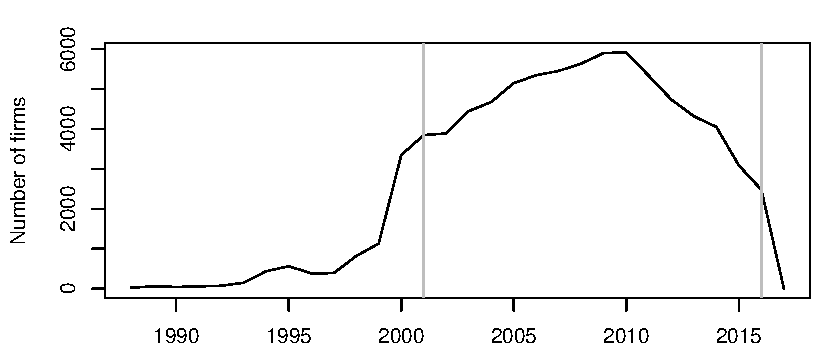
\includegraphics{./TABLES/compnfirms.pdf}
\caption{Number of firms by year}
\label{compnfirms}
\end{figure}
\end{center}
 In Prowess, firms
are under no legal obligation to report their finances, and hence it
is difficult to identify entry and exit of firms. Therefore in this
paper, I do not analyse the effect of export and import on
the survival probability of firms. The non-compulsory disclosure also
creates a bias in favour of large and publicly listed firms. However,
since exporters and importers are generally large, the results could
be biased downwards. 

I create two additional variables \textit{Export Value} and
\textit{Import Value}
% , and
% \textit{Domestic Sales}
by adding the following variables from Table \ref{indicator}.  
\begin{enumerate}
\item Export Value: Sum of the exports of goods and services (\textit{sa\_export\_goods $+$ sa\_export\_serv})
\item Import Value: Sum of imports of raw materials, stores and spares,
  finished goods and capital goods (\textit{sa\_import\_rawmat $+$        sa\_import\_stores\_spares
  $+$ sa\_import\_fg            $+$sa\_import\_cap\_goods})
% \item Domestic Sales: Total Sales - Export Sales( \textit{sa\_sales $-$ Export Value})
\end{enumerate}
Using these value variables, I create dummies for trade market
participation as follows:
\begin{itemize}
\item Export Dummy: $d_{it}^{X}=1$ if \textit{Export Value} $> 0$,
  otherwise $0$
\item Import Dummy: $d_{it}^{M}=1$ if \textit{Import Value} $> 0$, otherwise $0$
\end{itemize} 

Finally, I divide firms in the dataset into the following four categories:
\begin{itemize}
\item None: Firms that do not participate in the export and import
  market 
\item Export only: Firms that participate in the export market only
\item Import only: Firms that participate in the import market only
\item Both: Firms that participate in both export and import market
\end{itemize}

Table \ref{comp_table} displays the composition of firms according to their trade market
participation status. The number of firms that do not
participate in the trade market is low, around 20 to 35
\%. Surprisingly, the number of firms that participate in the trade
market is as high as 75\%. Another interesting feature is that the number
of firms that participate only in the import market is higher than the
firms that participate only in the export market. This can mean that
the demand for foreign intermediaries is relatively high. Also, almost 50 \% of
firms in each year participate in both export and import market. There is
a very high proportion of firms that participate in the both the trade market activities relative to the firms that
participate only in one trade market activity. 

\begin{center}
\input{./TABLES/composition.gen}
\end{center}
\section{Descriptive Statistics}\label{sec:desc}
\subsection{Exporter and Importer Performance}
To see the difference in performance of firms that participate in the trade market
versus those that don't, I show the density plots for log of sales, gross fixed assets,
salaries and for the four categories of 
firms trade behavior defined above, in  
Tables \ref{lsales}, \ref{lgfa} and \ref{tab:lsalary}, respectively. 
\newpage
 \newgeometry{ top=2cm}
\begin{center}
\begin{table}[H]
\caption{Summary Statistics of Sales (log)}
\label{lsales}
\begin{tabular}{c}
 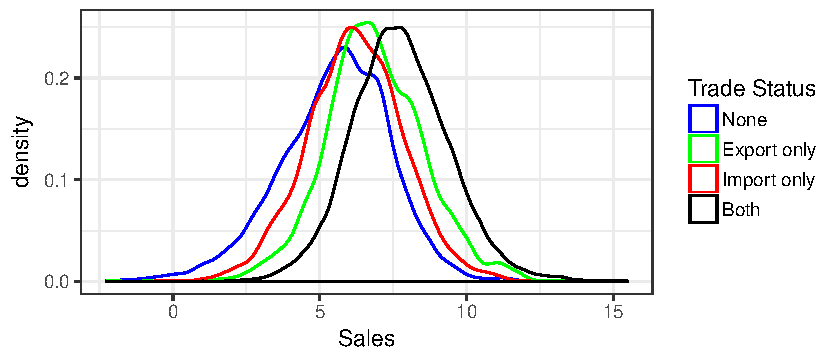
\includegraphics{./PICS/denslsales.pdf}   \\ 
 \input{./TABLES/sumstatslsales.gen}  \\  
\end{tabular}
\end{table}
\end{center}
\begin{center}
\begin{table}[H]
\caption{Summary Statistics of Gross Fixed Assets (log)}
\label{lgfa}
\begin{tabular}{c}
 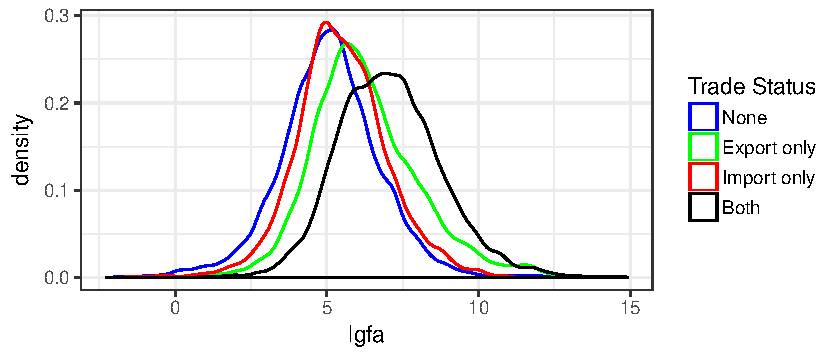
\includegraphics{./PICS/denslgfa.pdf}   \\ 
 \input{./TABLES/sumstatslgfa.gen}  \\  
\end{tabular}
\end{table}
\end{center}
 \restoregeometry



\begin{center}
\begin{table}[H]
\caption{Summary Statistics of Salary (log)}
\label{tab:lsalary}
\begin{tabular}{c}
 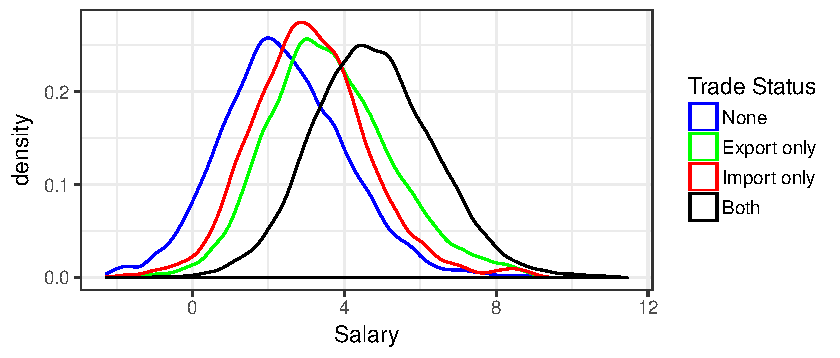
\includegraphics{./PICS/denslsalary.pdf}   \\ 
 \input{./TABLES/sumstatslsalary.gen}  \\  
\end{tabular}
\end{table}
\end{center}

The distribution of firms that participate in the trade market is more skewed towards the right for all the
variables mentioned above. In the case of sales, firms in category
`None' have an average of 5.52 whereas firms in category `Export Only';
and `Import Only' have and average  of 6.86 and
6.82 respectively. Moreover, firms in category `Both' have an average
of  7.74.  On the other hand, the standard deviation in the 4 
cases is very similar, which suggests that the increase in average is
not due to the presence of outliers. The same pattern is observed for
gross fixed assets and salary.  

This suggests that firms that participate in the both export and import market have
higher sales, mean gross fixed assets and 
salaries  than firms that participate in
only export and only import.  And firms that participate in either the
export or import market have higher values  than firms that do not
participate in the trade market. This indicates that firms participating
in the trade market has an positive effect on the observable
characteristics of the firm.

The same pattern in observed for expenditure on raw material (Table \ref{tab:lrawmat}) and
expenditure on power and fuel (Table \ref{tab:lfuel}) in the Appendix
section \ref{sec:fuel}
\subsection{Trade Premia}
Trade premia is defined as the difference in
attributes of firms based on their trade participation status. I
estimate the trade premia using the following Fixed Effect (FE) regression:
\begin{equation}
\label{FE}
 X_{it} = \alpha_i + \gamma_{t} + \beta_{1} d_{it}^{X}+ \beta_{2} d_{it}^{M}+
\beta_{3} d_{it}^{X}*d_{it}^{M} + \beta_{4} age_{it} + \epsilon_{it}
\end{equation}
where $X_{it}$ is firm level characteristics such as Sales, Gross
Fixed Assets, Expenditure on Raw Material and Salary, $d_{it}^X$ is
the export dummy, $d_{it}^M$ is
the import  dummy, the interaction term between these two variables
and $age_{it}$ is the age of the firm. I estimate this equation using
time and firm fixed
effects to account for time invariant firm characteristics, and any
time-specific effects.

%  This model is log-linear in nature. Therefore,
% if firm is exporting than it raises the dependent variable by
% $(exp(\beta) -1) 100$

\begin{center}
\input{./TABLES/expimppremia.gen}
\end{center}

Table \ref{expimppremia} displays the results for the above
regression. The coefficients for both export and import dummy are positive
and significant at 1\% significance level. Column 1 of this table
shows the trade premia for the variable sales. Firms
in category `Export Only'   52 \% $(exp(0.422) -1)* 100 = $ more
sales than firms `None'. Similarly firm in category `Import Only'
on average 54\% higher sales than firms in category `None'. 

 The interaction term value of $-0.060$ is not higher than the coefficient
value of the export and import dummy. Therefore, the cumulative
effect of participating in both activities is higher than the effect
of participating in just one trade activity. Therefore, firms that lie
in category `Both' have  on average 120\% higher sales than firms that
lie in category `None'. 

 The same trend
is also observed for  gross fixed assets, salary and expenditure on
raw materials.  The age variable also
has a positive coefficient and is significant at 1\% significance
level. Therefore,  on average the older a firm becomes the higher its capital,
assets etc. become. 

This section verifies the presence of trade premia in our
dataset. It further substantiates the point that firms that
participate in one trade market activity (export or import) have
better sales, gross fixed assets etc than firms that do not
participate in the trade market. Furthermore, firms that participate
in the both of the trade market activities have a higher trade premia
than the firms that participate in one of the trade activities. 

In the next section, I descriptively investigate whether exports have an effect
on imports and vice-versa.  

\subsection{Complementarity between Exporting and Importing}
The difference between density plots for export value of firms that
lie under category `Both'  versus those that lie in `Export Only' will
give a better understanding of whether there is an effect of one activity on the other. 
Table \ref{tab:lexport} displays the the density plot  of the log
values of export for firms in the category `Export only' and `Both'
defined above. The table shows that firms in category 'Both'
 have a higher mean of exports (5.24) than firms in category 'Export
 Only' (3.56). This suggests that importing may have a
positive association with exporting such that firms export more if
they also import.

Table \ref{tab:limport} displays the density plot of the log value of
import  for firms in category 'Both' and `Import Only'.
Firms that participate in both the
export and import market have higher imports (4.95) than firms that only
participate in the import market (3.41). Again, this shows that firms
import more if they are also exporters. 
% \newgeometry{top=3cm}
\begin{center}
\begin{table}[H]
\caption{Summary statistics of Export (log)}
\label{tab:lexport}
\begin{tabular}{c}
 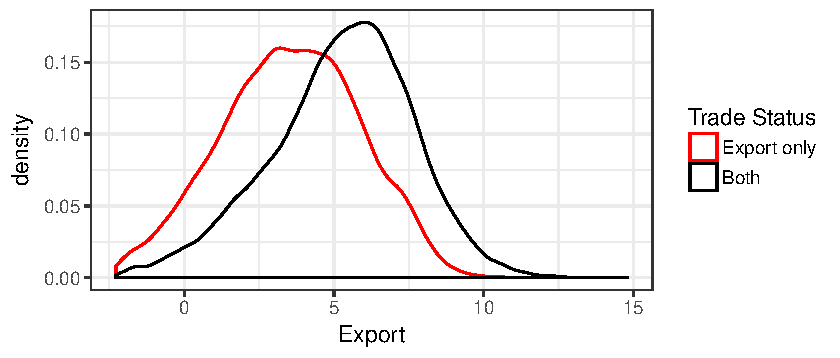
\includegraphics{./PICS/denslexport.pdf}   \\ 
 \input{./TABLES/sumstatslexport.gen}  \\  
\end{tabular}
\end{table}
\end{center}

\begin{center}
\begin{table}[H]
\caption{Summary statistics of Import (log)}
\label{tab:limport}
\begin{tabular}{c}
 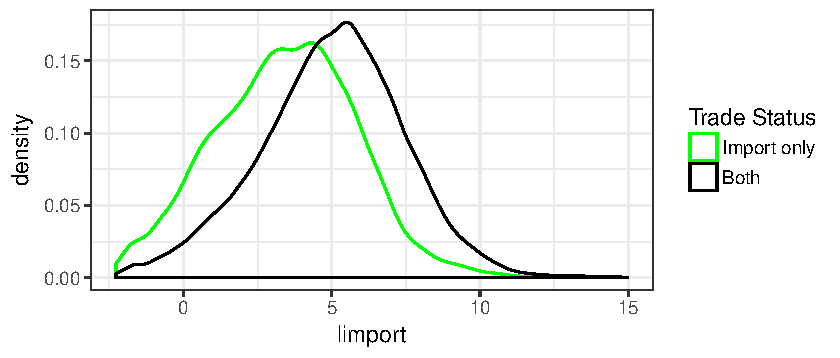
\includegraphics{./PICS/denslimport.pdf}   \\ 
 \input{./TABLES/sumstatslimport.gen}  \\  
\end{tabular}
\end{table}
\end{center}
% \restoregeometry

Tables \ref{tab:lexport} and \ref{tab:limport} suggest that both these activities have a
positive effect on the other and this might be because importing
complements exporting and vice-versa. This complementarity needs
further research, and is the focus of my paper. 

I estimate the trade premia similar to the regression in equation
\ref{FE} to see the effect decision to import on exporting value. This is done by estimating the
following fixed-effects (FE) regression:

$$  log(Export)_{it} = \alpha_{i} + \gamma_{t} +  \beta_{1} d_{it}^{M}+
+ \beta_{2} age_{it} + \epsilon_{it}$$

$$  log(Import)_{it} = \alpha_{i} + \gamma_{t} + \beta_{1} d_{it}^{X} + \beta_{2} age_{it} + \epsilon_{it}$$ 

\begin{center}
\input{./TABLES/prodpremia.gen}
\end{center}

The first two columns of table \ref{prodpremia} display these
results. Firms that  import have on average a higher value of exports. The
opposite is also true,
exporting firms have a higher value of imports.  This further suggests the presence of complementarity
between exporting and importing. 

In the next section, I investigate the effect of exporting and importing on
simple measures of productivity.
 
\subsection{Productivity and Export/Import}

\textcite{gupta2018exporting} define a simple measure of productivity known
as \textit{capital productivity}. It is defined as the log of value added per
unit of capital used by a firm:
\begin{equation}
 log(VA_{it}) - log(k_{it})
\end{equation}
where $VA_{it}$ is firm-level value added, computed as total industrial sales plus
change in stock minus power and fuel expenditures, and raw material
expenses. 
 Table \ref{tab:capprod} displays the summary statistics for this variable
based on the trade activity status. The mean of capital
productivity increases as activity status moves from \textit{None} to
\textit{Export only or Import only} to \textit{Both}, whereas the
standard deviation decreases.  
\begin{center}
\begin{table}[H]
\caption{Summary statistics of Capital Productivity (log)}
\label{tab:capprod}
\begin{tabular}{c}
 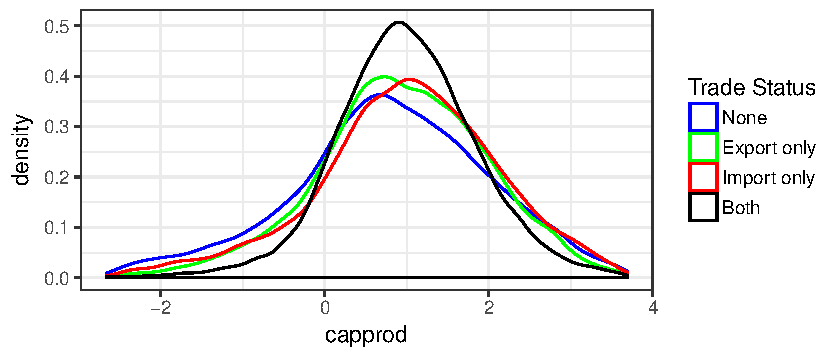
\includegraphics{./PICS/denscapprod.pdf}   \\ 
 \input{./TABLES/sumstatscapprod.gen}  \\  
\end{tabular}
\end{table}
\end{center}

%% TDDO: Revise
  Table \ref{tab:capprod} displays that firms which participate in
the trade market  have a higher  capital productivity as firms
participating in the trade market have a higher mean than those firms
that do not particii.epate in the trade. 

\begin{center}
\begin{table}[H]
\caption{Summary statistics of Profit to Sales}
\label{tab:pts}
\begin{tabular}{c}
 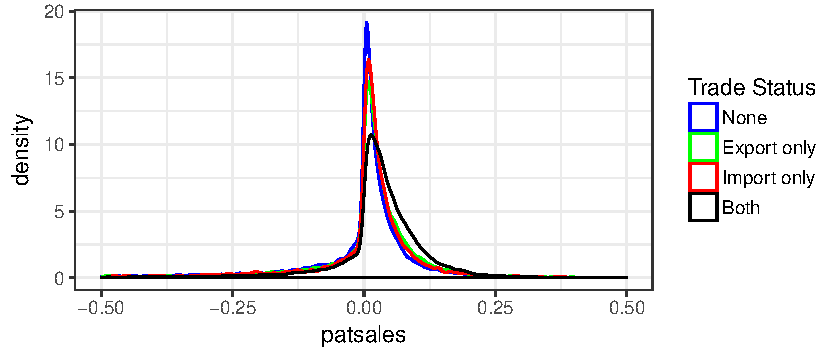
\includegraphics{./PICS/denspatsales.pdf}   \\ 
 \input{./TABLES/sumstatspatsales.gen}  \\  
\end{tabular}
\end{table}
\end{center}

I also use a measure of firm profitability, calculated by dividing the profit
after tax of
a firm with its sales. Table \ref{tab:pts} shows the summary
statistics for this variable. The same pattern is observed for this variable as well. The mean increases from -0.1 when a firm is not participating in
the trade market to -0.03 and  -0.06 when a firm is participating in
import and export respectively to 0.01 when a firm is participating in
both of the trade market activities.  

The last two columns of table \ref{prodpremia} estimate the trade
premia for the simple measures of the productivity defined above i.e
capital productivity and profit-to-sales ratio. Both
of the crude measures of productivity are positively correlated to the discrete
decisions of importing and exporting.  Firms under category `Export
Only' have on average a  higher
capital productivity and profit-to-sales ratio than firms under
category `None'. The same is also observed for firms under category
`Import Only'.
  
 The interaction term is lower than the coefficient of export and
 import column 3 and 
is not significant in column 4. This suggests firms under category
`Both' have on average a higher capital productivity and profit-to-sales ratio than
firms under category `Export Only' and `Import Only'. 

\subsection{Transition Probability}
%% change title


Table \ref{tab:transition} displays the transition probabilities
observed in the data  and the values in the brackets represent the
number of firms.  There are very high levels of persistence from
\textit{None} in t-1 to \textit{None} in t. Moreover,   high levels of persistence
are also observed in  \textit{Both}  (91.5\%). This means that there must be high sunk
costs to enter in the export and import market since only 12\% of the
firms  that do not participate in the trade market in t-1 start
participating in the trade market in t.

Interestingly, the levels of
persistence in \textit{Import Only} and \textit{Export Only}  is not
as high. A large portion of firms switch to participating in both the trade market
activities in period t. This suggests that participating in export in time
period in t-1 increases the probability of participating in import  markets in time period
t and vice-versa. Also, the number of firms that flip-flop (switch
trade market status) is low, which provides further evidence of sunk costs
to participating in the trade market as well. 

\begin{table}[H]
\begin{center}

\caption{Empirical Transition Probability}
\label{tab:transition}
\input{./TABLES/transition.gen}
\end{center}

\end{table}


This section provides descriptive evidence that firms that participate
in the trade market are bigger, and have higher
productivity than firms that do not participate in the trade
market. It provides evidence that exporting firms export more if they
participate in the import market as well and vice-versa. It also
provides evidence that there is persistence in trade status
(especially when the firms are not participating in the trade market
and when they are participating in the export and import market). 

In the next section, I proceed to calculate productivity using more
sophisticated techniques used in the literature and investigate the endogenous effect
of the decision to export and import on productivity. Then, I investigate if the
sunk cost hypothesis and self-selection hypothesis is observed using a
dynamic random effects probit model. I end the next section by
estimating a dynamic bivariate probit model to examine the complementary
nature of these two activities. 

\section{Empirical Analysis}\label{sec:anal}

The empirical analysis in this section is divided into the  following three
parts:
\begin{itemize}
\item Learning-by-Doing: How does lagged choice of export and import
  impact productivity?
\item Self-Selection and Sunk Cost Hypothesis:
\begin{itemize}
\item  Do  more productive firms self-select into
  exporting and importing and does the behavior of exporting and
  importing suggest the presence of a sunk cost? 
\item Lagged Cost Complementarity between Exporting and Importing:
  Does  engaging in one activity at time $t-1$
  increase the probability of engaging at time $t$ in the other?
\end{itemize}
\item Contemporaneous Cost Complementarity between Exporting and Importing : Does engaging
  in one activity at time $t$ complement participation in the other at
  time $t$?
\end{itemize}
%% TODO: Here lagged and comtemporaneous does not make sense to me immediately

\subsection{Learning-by-Doing}\label{sec:lbd}

 I assume that the firms have a Cobb-Douglas
production function: 

\begin{equation}
y_{it} =   \beta_{l}l_{it} + \beta_{k}k_{it} +
\omega_{it} + \eta_{it} 
\end{equation}
where $l_{it}$ is the labor, $k_{it}$ is capital, $\omega_{it}$ is the
total factor productivity or unobserved productivity and $\eta_{it}$
is a unknown shock affecting the firms output. However, the OLS
estimation provides biased results as it does not account for
simultaneity problem i.e the productivity of a firm should be
correlated with the inputs of production. 

There is a vast literature on the estimation of productivity starting
with the seminal paper in productivity estimation: \textcite{olley1992dynamics} and subsequent
modifications of their method: \textcite{levinsohn2003estimating},
\textcite{ackerberg2006structural} and
\textcite{wooldridge2009estimating}. The estimation strategy of
\textcite{olley1992dynamics} is highlighted in section \ref{op}. 
%% TODO: Then why do you describe OP in the appendix. You should also
%% mention some reasons for why you use LP and ACF. OP uses investment
%% as an instrument and there are many zeroes for this variable in
%% Prowess, so LP makes more sense.

\textcite{olley1992dynamics} \textbf{OP} uses investment
 as function of productivity and capital to invert out productivity.  There are many zeroes for this variable in
 data. Therefore, I use the  methods shown in \textcite{levinsohn2003estimating} and
\textcite{ackerberg2006structural} to estimate Cobb-Douglas
parameters as they use  intermediate
input demand instead.  


\textcite{levinsohn2003estimating} \textbf{LP} uses a  strategy
similar to \textcite{olley1992dynamics} but use intermediate input demand
as the function to invert out $\omega_{it}$. 
Here, the intermediated material demand function is given by:
$$  m_{it} = m_{it}(\omega_{it}, k_{it})$$
This function is assumed to be montonically increasing and therefore
productivity can be found by inverting the function above. Therefore,
we can write the Cobb-Douglas equation  as: 
$$ y_{it} = \beta_{l}l_{it} + \phi_{it}(m_{it},k_{it})$$
where $\phi_{it}(m_{it},k_{it}) =  \beta_{k}k_{it}+ \omega_{it}(m_{it}, k_{it})$
. They suggest the  use of a third degree polynomial to approximate 
$\phi_{it}$ and substitute it into the equation above to give the
following result: 

$$  y_{it} =  \beta_{l}l_{it} + \sum_{i=0}^{3} \sum_{j=0}^{3}
\delta_{ij}k_{it}^{i}m_{it}^{j} + \eta_{it}$$
The coefficient is $\beta_{l}$ is estimated by OLS using the equation
above as they assume that the labor is a flexible input i.e there are
no labor adjustment costs and $\hat{\phi}_{it}$ is estimated by
subtracting the effect of labor from
the fitted value of the previous equation:

%% TODO: Instead of saying above, try to number your
%% equations. `Above' makes it confusing. If it is the previous
%% statement, say that.

$$ \hat{\phi}_{it} = \hat{y}_{it} - \hat{\beta}_{l}l_{it} =
 \sum_{i=0}^{3} \sum_{j=0}^{3}
\hat{\delta_{ij}}k_{it}^{i}m_{it}^{j}$$
Therefore,  for any value of $\beta_{k}$:
$$\hat{\omega}_{it} = \hat{\phi}_{it} - \beta_{k}k_{it}$$
 It is also assumed that $\omega_{it}$ follows a first order Markov
process : 
$$\omega_{it} = E[\omega_{it}|\omega_{it-1}] + \epsilon_{it}$$
They  assume a polynomial expansion of the expectation above to give:
$$ \omega_{it}=  \gamma_{o}+\gamma_{1}\omega_{it-1} +
\gamma_{2}\omega_{it-1}^2 + \gamma_{3}\omega_{it-1}^3 + \epsilon_{it} $$ 
Therefore, the value of $\beta_{k}$, for which the expression below is
minimised is chosen to be the coefficient of capital.  
\begin{equation}
\beta_{k}^{*} = arg \underset{\beta_{k}}{\min}\sum_{i=1}^{N}\sum_{t=2}^{T} (y_{it} - \hat{\beta_{l}}l_{it} -
\beta_{k}k_{it} - \hat{E[\omega_{it}|\omega_{it-1}]})^2 
\end{equation}

On the other hand, \textcite{ackerberg2006structural} \textbf{ACF} use a
similar strategy but, suggest that labour might also be
correlated with productivity. Therefore, they write  the firms input
material demand as a function of productivity, capital as well as
labor : 
$$ m_{it} = f_{it}(\omega_{it}, k_{it}, l_{it})$$
Inverting this function for $\omega_{it}$ and substituting into the
production function results in the following 
equation of the form:
\begin{equation}
y_{it} = \beta_{l}l_{it} + \beta_k k_{it} + f_{it}^{-1}(m_{it},
k_{it}, l_{it})+ \epsilon_{it}
\end{equation}


They suggest that the  labor coefficient along with capital since it is correlated with
productivity. 
%% TODO: This sentence is not very clear!

They suggest the following steps:
\begin{enumerate}
\item Obtain $\phi_{it}(m_{it}, k_{it}, l_{it}) = \beta_{l}l_{it} + \beta_k k_{it} + f_{it}^{-1}(m_{it},
k_{it}, l_{it})$ by regressing $y_{it}$ on polynomial approximation of
$\phi_{it}(m_{it}, k_{it}, l_{it})$
\item Use the Markovian nature of $\omega_{it} =
  E(\omega_{it}|\omega_{it-1}) + e_{it}$
and use the following moment equations to estimate $\beta_{k}$ and
$\beta_{l}$:
\begin{equation}
E[e_{it}(\beta_{k},\beta_{l})|\begin{pmatrix}k_{it}\\ l_{it-1}
\end{pmatrix}
]= 0
\end{equation}
\end{enumerate} 
%% TODO: There is only one moment condition. How will you estimate two
%% parameters from only one moment condition: There are two k_{it} and l_{it-1}

%% TODO: Cite a paper in the paragraph below: I cite the DeLocker paper

However, exogenously regressing lagged  export and import variables  on
productivity (residuals of the Cobb-Douglas function) suggests that past
export and import performance  does not impact future revenue and the
capital coefficient will be biased if capital is correlated with the
export or import status.  This has been highlighted by \textcite{de2013detecting}, and
they suggest that the trade activities should be accommodated
endogenously in the productivity evolution process. This is done by
accommodating the the lagged export and import variable into the
Markovian productivity evolution procedure:
%% TODO: Explain this a bit more!

$\omega_{it} =
  E(\omega_{it}| \omega_{it-1}, d_{it-1}^{X}, d_{it-1}^{M}) + e_{it}$

% \subsection{Learning-by-doing}


% I estimate the  endogenous  effect of export/import on productivity
% using two techniques  used widely in this field: 
%  \textcite{levinsohn2003estimating} (LP)and
%  \textcite{ackerberg2006structural} (ACF).
% ACF results are shown to highlight the robustness of the results. 
% \subsubsection{Levinsohn-Petri}
% \textcite{levinsohn2003estimating} assume the following  Cobb-Douglas production function: 
% \begin{equation}
% y_{it} = \beta_{o} + \beta_{l}l_{it} + \beta_{k}K_{it} +
% \omega_{it}(m_{it}, k_{it}) + \eta_{it} 
% \end{equation}

% Using OLS residuals of the Cobb-Douglas estimates provide biased
% estimates of productivity since there is correlation between
% productivity and characteristics  of firms.   

I use the log values of the following variables for the estimation
procedure:  gross fixed assets as a measure of capital, salary
as a measure of labor and a expenditure on raw materials as a measure
of intermediated input. Since productivity evolution is  assumed to
have a Markovian nature, I assume the following form of productivity
evolution where it depends upon  the discrete decision to export and import:
%% TODO: Shouldn't it be `since evolution of productivity is
%% markovian': I dont think it matters that much 

\begin{equation}
 \omega_{it} = \alpha_{o} + \alpha_{1}\omega_{it-1} +
\alpha_{2}\omega_{it-1}^{2} + \alpha_{3}\omega_{it-1}^{3}+
\alpha_{4}d_{it-1}^{X} + \alpha_{5} d_{it-1}^{M} +
\alpha_{6}d_{it-1}^{X}d_{it-1}^{M}  + \nu_{it}
\end{equation} 
where $d_{it-1}^{X}$ and $d_{it-1}^{M}$ is the discrete decision to
export and import respectively. 

I report the estimates for the effect of discrete decision to export
and import on productivity in the main section whereas I report the
effect of the log values of export and import on productivity the
appendix section \ref{apendix:lbd}.  

The estimates of the Cobb-Douglas and  the productivity evolution
coefficients  using the Levinsohn-Petrin
method are shown in Table \ref{regLP} and \ref{prod}  respectively. 
\input{./TABLES/regLP.gen}
\input{./TABLES/prod.gen} 
Table \ref{prod} shows that coefficients of $\omega_{it-1},
\omega_{it-1}^{2}$ and $\omega_{it-1}^{3}$ are significant at 1\%. Therefore, productivity evolutions depends strongly
on the past productivity and the coefficients suggest that there is a
non linear relationship with past
productivity. The coefficient of $d_{it-1}^{X}$ is positive but it is
not significantly different than zero and  coefficient of
$d_{it-1}^{M}$  is positive and significant at 1\% level. The
interaction term between exporting and importing also does not have a significant effect on productivity.
The results suggest lagged decision to export does not a have
a significant effect on productivity (firms do not experience learning-by-exporting). However, 
lagged decision to import causes the productivity to increase by 3.5  per
cent (firms experience learning-by-importing).  


Table \ref{regLPcont} and \ref{prodcont} in the Appendix \ref{apendix:lbd} display the Cobb-Douglas and
productivity evolution
coefficients  when the
productivity evolution is dependent on the lagged continuous log value of export
and import rather than the lagged decision to export and import.
The effect of export and import has the same sign in this case as
well. It shows that lagged
continuous value of export does not have a significant effect on
productivity and  increase in lagged continuous log value of import  by 1 unit
increases the productivity by 3.6 \%.  
%% TODO: WHy is this table in the appendix? This is a robustness
%% check. And all of my results are for the decision to export and import
%% and not the value exported/imported. 


As written before, \textcite{de2013detecting} say that exogenously accommodating the
decision to export and import implies that
past export and import experience has no impact on direct technological
improvements. Therefore, the coefficient of capital will be biased
upwards if the decision to participate in the trade market correlated with capital. Table
\ref{regLPex} displays the coefficients when the export and import
decision is not endogenously accommodated in 
productivity evolution. In this case, the coefficient of capital is
biases upwards (0.452 (Table \ref{prodcont}) compared to 0.437 (Table \ref{prod}) the endogenous case)  since
the variation in output is attributed more towards capital rather than productivity.   
\input{./TABLES/regLPex.gen}
%% TODO: I have edited the last sentence. Is this what you were trying
%% to say?
%% TODO: Say where 0.452 number is and in which table 0.437 is. It was
%% not clear to me that 0.437 is the endogenous estimation table.

% \subsubsection{\textcite{ackerberg2006structural}}
The results from the estimation method mentioned in
\textcite{ackerberg2006structural} \textbf{ACF} are shown in \ref{regACF} and \ref{prodACF}. The coefficient of labor is similar in this
estimation method which further suggests that labor is a flexible
input as assumed in the \textbf{LP} estimation procedure. The results also
show strong dependence on past productivity. In terms of the endogenous effect
of export and import on productivity is roughly the same. The export
decision does not have a significant effect on productivity and the
import decision has a 2.6\% increase to the productivity. These
results are similar to the results from the Levinsohn-Petrin
estimation.   %% TODO: Mention the right table to look at: It is the
              %% right table 
 
 

\input{./TABLES/regACF.gen}
\input{./TABLES/prodACF.gen}

Tables \ref{regACFcont} and \ref{prodACFcont} in Appendix \ref{apendix:lbd}  display the Cobb-Douglas and
productivity evolution
coefficients,  when the
productivity evolution is dependent on the lagged continuous lag value of
export and importing. The results also show a similar effect of export
and import on productivity as the discrete choice results.  
%% TODO: I think before you do the four estimations, write a paragraph
%% which tells the reader what you will be doing in the rest of the
%% subsection. The difference between using discrete and continous
%% value of exporting and importing was not clear to me since you did
%% not mention that in the section where you talk about the different
%% estimation procedures.

A drawback of this estimation procedure is that 
the Cobb-Douglas production function used in the estimation procedure  does not
account for immediate impact (effect at time t) of 
importing behavior to the productivity of a firm.  It is assumed that
participating in the import market has an effect only in increasing the
productivity of the firm in the next period (at time t$+$1). 

%% TODO: Do you know how to account for this drawback, or can you cite
%% someone who has done it. If not, say that a model that accounts for
%% comtemporaneous effects is
%% beyond the scope of this paper.: I do not know how to account for
%% this drawback. How do I say that I do not know how to account for
%% this?

Based on the results above,  I conclude that manufacturing firms experience learning-by-importing and
do not experience learning-by-exporting. 
In the next section, I investigate if more productive firms self-select into
exporting and importing and if the sunk cost hypothesis is observed for
the discrete decision to export and import with the help of a dynamic probit
random effects model. 
% \newpage
\subsection{Sunk Cost and Self-Selection Hypothesis }\label{sec:ss}

%% TODO: Here you should state the sunk cost hypothesis also.
The sunk cost and self-selection hypothesis states that entry into the trade market
involves   costs that are sunk in nature and only the most productive firms can
overcome these trade costs. To investigate this hypothesis, I
estimate a dynamic random effects probit model similar to the model used
in \textcite{roberts1997decision}. I define $d_{it}^{X}$ as the discrete
decision to export, where
 Bellman equation for a profit maximising firm deciding to enter the
 export market is:
 %% TODO: Does your analysis differ from roberts paper? Say so: It
 %% does not differ that much. What do I do in that case?

 
\begin{equation}
V_{it}(S_{it})= \underset{d_{it}^{X}}{\max}\:  \mathbb{E}_{t}(\sum_{i=0}^{\infty} \delta^{t+i}R_{i,t+i}|S_{it})
\end{equation}
 where $\delta$ is the one-period discount factor, $S_{it}$ is the
 relevant state variables affecting the firms decision, $R_{it}$ is
 the revenue. Expanding the profit for time $t$, the equation above can also be written as:
 %% TODO: I have rewritten the last line, check if it makes sense
 
\begin{equation}
V_{it}(S_{it})= \underset{d_{it}^{X}}{\max} (\pi^{D}(S_{it}) + d_{it}^{X}(\pi^{X}(S_{it})- f^{X} -
c^{X}(1-d_{it-1}^{X}))  + \sum_{t=t11}^{\infty} \delta^{t-j}R_{ij}|S_{it})
\end{equation}

where $\pi^{D}(S_{it})$ is the domestic profit, $\pi^{X}(S_{it})$ is the export
profit, $f^{X}$ is the fixed cost of exporting and $c^{X}$ is the sunk
cost of exporting. This equation can also be written as:
\begin{equation}
V_{it}(S_{it})= \underset{d_{it}^{X}}{\max} \:\mathbb{E}
\Big(\pi^{D}(S_{it}) + d_{it}^{X}(\pi^{X}(S_{it}) - f^{X} -
c^{X}(1-d_{it-1}^{X}))  + \delta \mathbb{E} (V_{it}(S_{it+1})|S_{it},
d_{it}^{X}) \Big)
\end{equation}

 Thus, a firm will participate in the export market if:
\begin{equation}
\begin{aligned}
\pi_{it}^{*} = \pi^{X}(S_{it})  +
\delta \mathbb{E}_{t}(V_{i,t+1}(S_{it+1}|S_{it},d_{it}^{X}=1) -
V_{i,t+1}(S_{it+1}|S_{it},d_{it}^{X}=0))\\ 
-  (f^{X} +
c^{X}(1-d_{it-1}^{X})) \geq 0
\end{aligned}
\end{equation}

It is assumed that the state variables entering the Bellman equation
are the following: $S_{it}= (k_{it}, l_{it}, \omega_{it},
d_{it-1}^{X})$ i.e capital, labor, productivity and lagged decision to
participate in the export market. In the model above, it is assumed
that a firm pays a sunk cost if it did not participate in the export
market in the previous period  ($d_{it-1}^{X} = 0$).  If there are no sunk costs, then
according to the Bellman equation above, a firm will export as long as
the current profits plus the discounted expected profit is greater
than the fixed costs of exporting. 
The reduced form expression of the equation above is: 
\begin{equation}
  d_{it}^{X}=\begin{cases}
   1 , & \text{if $\pi_{it}^{*} \geq 0$}.\\
   0 , & \text{if $\pi_{it}^{*}<  0$}.
  \end{cases}
\end{equation}

To do the reduced form estimation of the model, I write the above equation as a linear
function of the relevant state variables mentioned in the previous
paragraph, along with dummy variables to
adjust for industry and time effects as follows:

\begin{equation}
\label{eq:export}
  \pi_{it}^{*}=   \gamma_{1}^{X} d_{it-1}^{X} + 
\gamma_{3}^{X} \hat{\omega}_{it}  + \beta_{1}^{X}k_{it}  +\beta_{2}^{X}l_{it}+
s_{i}^{X} + \mu_{t}^{X}  + \alpha_{i}+ \epsilon_{it}^{X}
\end{equation}
%% TODO: Explain what the variables mean. Or atleast say as defined in
%% section bla bla: I have defined them in the previous paragraph
%% where I display the relevant state variables. 


A positive and significant coefficient for $d_{it-1}^{X}$ shows that there is
persistence in exporting behavior, and thus provides
evidence for the presence of sunk cost in export market participation.
If the sunk cost hypothesis did not hold then the probability of exporting
should not depend on the lagged decision to export. Moreover, a positive and significant
coefficient for $\omega_{it}$  provides evidence for the
self-selection hypothesis as firms with high
productivity have a higher probability of participating  in the export
market. Finally, a positive and significant coefficient for $k_{it}$
and $l_{it}$ provides evidence indicating that bigger firms have a
higher chance of participating in the export market. 


A similar model can be estimated for the discrete decision to import,
since importing also involves additional fixed and sunk costs. A firm
would be able to participate in the import market if the productivity
benefits are enough to overcome the costs. Learning-from-importing has already been
demonstrated in the previous section. The Bellman equation of a firm
deciding to enter the import market is the following: 

\begin{equation}
V_{it}(S_{it})=  \underset{d_{it}^{M}}{\max}\Big(\pi(S_{it}) - d_{it}^{M}( f^{M} +
c^{M}(1-d_{it-1}^{M}))  + \delta \mathbb{E} (V_{it}(S_{it+1})|S_{it}, d_{it}^{M})\Big)
\end{equation}

where $\pi$ is total profit of a firm, $f^{M}$ is the fixed cost of
importing and  $c^{M}$ is the sunk cost of importing and  $S_{it} = (k_{it}, l_{it}, \omega_{it},
d_{it-1}^{M})$. 

Since $S_{it}$ contains productivity and the previous section suggests
that firms exhibit productivity improvements,  therefore,  this Bellman equation assumes that
importing in time t provides benefits in t+1 as the decision to
import increases the expected value productivity in the next period. Here, a firm will participate in the
import market if:

\begin{equation}
\begin{aligned}
\pi^{*}= 
\delta \mathbb{E}_{t}\Big(V_{i,t+1}(S_{it+1}|S_{it},d_{it}^{M}=1) -
V_{i,t+1}(S_{it+1}|S_{it},d_{it}^{X}=0) \Big) \\-  
(f^{M} + c^{M}(1-d_{it-1}^{M})) \geq 0
\end{aligned}
\end{equation}

Therefore, a firm will participate in the import market if the
discounted productivity benefits of participating in the
import market outweigh the costs of participating in it.
\begin{equation}
  d_{it}^{M}=\begin{cases}
   1 , & \text{if $\pi^{*} \geq 0 $}.\\
   0 , & \text{otherwise}.
  \end{cases}
\end{equation}

%% TODO:
                                %% Shown in equation bla bla: DOne

This can be tested with a reduced form dynamic probit model similar to
the discrete decision to export in equation \ref{eq:export}  Therefore, the reduced form equations of
the discrete choices to export and import are the following:

%% TODO: What is the base model? Base model is the model which
%% does not account for the lagged complementarity.

\begin{equation}
\label{eq:base1}
d_{it}^{X*} = \gamma_{1}^{X} d_{it-1}^{X} + 
\gamma_{3}^{X} \hat{\omega}_{it}  + \beta_{1}^{X}k_{it}  +\beta_{2}^{X}l_{it}+
s_{i}^{X} + \mu_{t}^{X}  + \alpha_{i}+\epsilon_{it}^{X}
\end{equation}
\begin{equation}
\label{eq:base2}
d_{it}^{M*} = \gamma_{1}^{M} d_{it-1}^{M} + 
\gamma_{3}^{M} \hat{\omega}_{it}  + \beta_{1}^{M}k_{it}  +\beta_{2}^{M}l_{it}+
s_{i}^{M} + \mu_{t}^{M}  + \alpha_{i}+\epsilon_{it}^{M}
\end{equation}
Here $s_{i}$ is a vector of industry dummies and $\mu_{t}$ is a vector
of time dummies. Equation \ref{eq:base1} and \ref{eq:base2} are
referred to as the \textit{Base Model}.  





%% TODO: Here explain the word lagged complemenratity

The \textit{Lagged cost complementarity} hypothesis states that the
decision to export at time $t-1$  could decrease the cost of importing at
time $t$ and vice-versa. To investigate the presence of lagged cost complementarity between exporting and
importing, I add another variable to the state space of the bellman equation: lagged export
decision into the import decision equation and lagged import decision
to export decision equation. Therefore, the  corresponding Bellman equation that
accounts for lagged complementarity for the export decision is: 
\begin{equation}
\label{eq:belllagex}
V_{it}(S_{it})= \underset{d_{it}^{X}}{\max} \Big(\pi^{D}(S_{it}) + d_{it}^{X}(\pi^{X}(S_{it})) - F(d_{it}^{X},d_{it-1}^{X}, d_{it-1}^{M})
  + \delta \mathbb{E} (V_{it}(S_{it+1})|S_{it}, d_{it}^{X}) \Big)
\end{equation}
where 
 
\begin{equation}
  F(d_{it}^{X},d_{it-1}^{X}, d_{it-1}^{M})=\begin{cases}
   \lambda^{X} * d_{it}^{X}( f^{X} +c^{X}(1-d_{it-1}^{X})), & \text{if $d_{it-1}^{M}= 1$}.\\
   d_{it}^{X}( f^{X} +c^{X}(1-d_{it-1}^{X})) , & \text{if $d_{it-1}^{M}= 0$}.
  \end{cases}
\end{equation}

% $F(d_{it}^{X},d_{it-1}^{X}, d_{it-1}^{M})$ is: 
% \begin{itemize}
% \item $\lambda^{X} * d_{it}^{X}( f^{X} +c^{X}(1-d_{it-1}^{X})$ \hfill for
%   $d_{it-1}^{M}= 1$
% \item $d_{it}^{X}( f^{X} +c^{X}(1-d_{it-1}^{X})$\hfill for
%   $d_{it-1}^{M}= 0$
% \end{itemize}

Here, $\lambda^{X}$ is the degree of cost complementarity that the
lagged decision to import has on the decision to export. If the value
of $\lambda^{X} > 1$, then participating in the import market in
period $t-1$ increases the cost to export in period t. If
$\lambda^{X}=1$, then participating in the import market in
period $t-1$ does not have an effect on the cost to export in period t.
If $0<\lambda^{X}< 1$,     then participating in the import market in
period $t-1$ decreases the cost to export in period t.


Similarly, the Bellman equation for the import decision is: 
\begin{equation}
V_{it}(S_{it})= \underset{d_{it}^{M}}{\max}\big(\pi(S_{it}) - F(d_{it}^{M},d_{it-1}^{M}, d_{it-1}^{X})  + \delta \mathbb{E} (V_{it}(S_{it+1})|S_{it}, d_{it}^{M})\Big)
\end{equation}
where 
\begin{equation}
  F(d_{it}^{M},d_{it-1}^{M}, d_{it-1}^{X})=\begin{cases}
   \lambda^{M} * d_{it}^{M}( f^{M} +c^{M}(1-d_{it-1}^{M})), & \text{if $d_{it-1}^{X}= 1$}.\\
   d_{it}^{M}( f^{M} +c^{M}(1-d_{it-1}^{M})) , & \text{if $d_{it-1}^{X}= 0$}.
  \end{cases}
\end{equation}
% where $F(d_{it}^{M},d_{it-1}^{M}, d_{it-1}^{X})$ is: 
% \begin{itemize}
% \item $\lambda^{M}  d_{it}^{M}( f^{M} +c^{M}(1-d_{it-1}^{M}))$ \hfill for
%   $d_{it-1}^{X}= 1$
% \item $d_{it}^{M}( f^{M} +c^{M}(1-d_{it-1}^{M}))$\hfill for
%   $d_{it-1}^{M}= 0$
% \end{itemize}

Here, $\lambda^{M}$ represents the degree of complementarity on the
cost to import if a firm participated in
the export market in the previous period. The reduced form
equation of the two Bellman equations that account for lagged
complementarity are the following:\\


\begin{equation}
\label{eq:lag1}
d_{it}^{X*}=   \gamma_{1}^{X} d_{it-1}^{X} + \gamma_{2}^{X} d_{it-1}^{M}+
\gamma_{3}^{X} \hat{\omega}_{it}  + \beta_{1}^{X}k_{it}  +\beta_{2}^{X}l_{it}+
s_{i}^{X} + \mu_{t}^{X}  + \alpha_{i}^{M}+ \epsilon_{it}^{X}
\end{equation}
\begin{equation}
\label{eq:lag2}
d_{it}^{M*}=   \gamma_{1}^{M} d_{it-1}^{M} + \gamma_{2}^{M} d_{it-1}^{M}+
\gamma_{3}^{M} \hat{\omega}_{it}  + \beta_{1}^{M}k_{it}  +\beta_{2}^{M}l_{it}+
s_{i}^{M} + \mu_{t}^{M}  + \alpha_{i}^{M}+ \epsilon_{it}^{M}
\end{equation}
Equations \ref{eq:lag1} and \ref{eq:lag2} are referred to as the
\textit{Lagged Complementarity Model}. 

Here, it is important to notice that  $\gamma_{2}^{X}$ measures the
cost complementarity effect of lagged importing on
exporting, since the productivity benefit of lagged importing
(learning-from-importing) is already
accounted for in $\hat{\omega}_{it}$. Therefore, if $\gamma_{2}^{X}>0$, then this means that
importing in time $t-1$ leads to decrease in cost of exporting at time t.  
Similarly, if  $\gamma_{2}^{M}>0$, then this means that
exporting in time $t-1$ leads to decrease in cost of importing at time
t. The interpretation of the other coefficients is the same as in
equations \ref{eq:base1} and \ref{eq:base2} respectively. 
%% TODO: Is the condition only >0 or also <1?: It is only > 0 as I am
%% only concerned with a positive value
  
I use a dynamic random effects probit specification with Wooldridge
method (\textcite{wooldridge2005simple}) which treats the initial conditions problem by accounting for
the correlation of the initial value of $d_{i1}$ with $\alpha$:
%% TODO: Elaborate a bit on this. Like what are you using the random effects model for. Why is this model appropriate?


$$  \alpha_{i}= \gamma d_{i1}+ \tilde{\alpha}_{i} $$
where $ \tilde{\alpha_{i}} \sim N(0, \sigma_{\alpha}^{2}) $

A random effects model is used because it accounts for the unobserved
individual heterogeneity and the methodology of
\textcite{wooldridge2005simple} helps to account for the correlation
between the initial value and the unobserved heterogeneity.\footnote{A
  brief description of the dynamic random effects probit model is
  provided in Appendix section \ref{apendix:random}.}
 
I use the log value of gross fixed assets as a measure of capital, log
value of wages as a measure of labor and use productivity estimates  of
the Levinsohn-Petrin method in the previous section along with
industry and time dummies.  
%% TODO: any reason you use LP, and not ACF estimation: Not any
%% particular reason. I just display one in the main section and the
%% other in the Appendix. 

Table \ref{tab:dynprobit} and \ref{tab:dynprobitme} shows the results of the 
estimation and the average marginal effects of the dynamic random
effects probit model, respectively. Columns 1 and 3 in both the tables show the result for the base
reduced model of importing and exporting  whereas columns 2 and 4
display the estimates when accounting for the lagged complementarity
between exporting and importing. 


\newgeometry{left= 2.5cm, top=4cm}
\begin{center}
\begin{table}[H]
\caption{Dynamic Random Effects Probit (Estimates)}
\label{tab:dynprobit}
{
\def\sym#1{\ifmmode^{#1}\else\(^{#1}\)\fi}
\begin{tabular}{l*{2}{c}}
\hline\hline
            &\multicolumn{1}{c}{(1)}&\multicolumn{1}{c}{(2)}\\
            &\multicolumn{1}{c}{exp}&\multicolumn{1}{c}{imp}\\
\hline
main        &                     &                     \\
lagexp      &       1.870\sym{***}&                     \\
            &     (77.04)         &                     \\
[1em]
L.lpres     &       0.173\sym{***}&       0.205\sym{***}\\
            &     (13.61)         &     (18.05)         \\
[1em]
L.lgfa      &      0.0856\sym{***}&       0.118\sym{***}\\
            &      (7.09)         &     (10.74)         \\
[1em]
L.lsalary   &       0.158\sym{***}&       0.157\sym{***}\\
            &     (12.48)         &     (14.21)         \\
[1em]
initexp     &       1.221\sym{***}&                     \\
            &     (29.21)         &                     \\
[1em]
lagimp      &                     &       1.648\sym{***}\\
            &                     &     (72.70)         \\
[1em]
initimp     &                     &       1.009\sym{***}\\
            &                     &     (28.73)         \\
[1em]
\_cons      &      -2.973\sym{***}&      -3.031\sym{***}\\
            &    (-15.67)         &    (-16.97)         \\
\hline
lnsig2u     &                     &                     \\
\_cons      &      -0.508\sym{***}&      -0.782\sym{***}\\
            &     (-8.66)         &    (-13.65)         \\
\hline
\(N\)       &       67591         &       67591         \\
rho         &       0.376         &       0.314         \\
sigma\_u     &       0.776         &       0.676         \\
\hline\hline
\multicolumn{3}{l}{\footnotesize \textit{t} statistics in parentheses}\\
\multicolumn{3}{l}{\footnotesize \sym{*} \(p<0.05\), \sym{**} \(p<0.01\), \sym{***} \(p<0.001\)}\\
\end{tabular}
}

\end{table}
\end{center}
\restoregeometry
\begin{center}
\begin{table}[H]
\caption{Dynamic Random Effects Probit (Average Marginal Effects)}
\label{tab:dynprobitme}
{
\def\sym#1{\ifmmode^{#1}\else\(^{#1}\)\fi}
\begin{tabular}{l*{4}{c}}
\hline\hline
            &\multicolumn{1}{c}{(1)}&\multicolumn{1}{c}{(2)}&\multicolumn{1}{c}{(3)}&\multicolumn{1}{c}{(4)}\\
            &\multicolumn{1}{c}{} &\multicolumn{1}{c}{} &\multicolumn{1}{c}{} &\multicolumn{1}{c}{} \\
\hline
lagexp      &       0.218\sym{***}&       0.212\sym{***}&                     &      0.0495\sym{***}\\
            &   (0.00410)         &   (0.00393)         &                     &   (0.00303)         \\
[1em]
lpres       &      0.0257\sym{***}&      0.0235\sym{***}&      0.0362\sym{***}&      0.0347\sym{***}\\
            &   (0.00161)         &   (0.00159)         &   (0.00165)         &   (0.00161)         \\
[1em]
lgfa        &     0.00797\sym{***}&     0.00553\sym{***}&      0.0142\sym{***}&      0.0130\sym{***}\\
            &   (0.00154)         &   (0.00151)         &   (0.00158)         &   (0.00153)         \\
[1em]
lsalary     &      0.0250\sym{***}&      0.0220\sym{***}&      0.0279\sym{***}&      0.0243\sym{***}\\
            &   (0.00164)         &   (0.00162)         &   (0.00161)         &   (0.00158)         \\
[1em]
lagimp      &                     &      0.0439\sym{***}&       0.209\sym{***}&       0.202\sym{***}\\
            &                     &   (0.00299)         &   (0.00389)         &   (0.00375)         \\
\hline
\(N\)       &       62485         &       62485         &       62485         &       62485         \\
\hline\hline
\multicolumn{5}{l}{\footnotesize Standard errors in parentheses}\\
\multicolumn{5}{l}{\footnotesize \sym{*} \(p<0.05\), \sym{**} \(p<0.01\), \sym{***} \(p<0.001\)}\\
\end{tabular}
}

\end{table}
\end{center}

% Therefore, I
% interpret the model which accounts for the lagged complementarity.
 
% \begin{enumerate}
% \item Export: \\$H_{o}$: Base Model, $H_{1}$:Model with lagged discrete
%   import variable.
% $LR= 2[ln(model2) - ln(model1)] = 2[-14406.6 + +14513.0] = 106.4$
% The critical value of $\chi^{2}_{1;0.95}= 3.84 $. Therefore $H_{o}$ is
% rejected. 
% \item Import:\\ $H_{o}$: Base Model, $H_{1}$:Model with lagged discrete
%   export variable. 
% $LR= 2[ln(model2) - ln(model1)] = 2[-15749.5 + 15879.7 ] = 130.19$
% The critical value of $\chi^{2}_{1;0.95}= 3.84 $. Therefore $H_{o}$ is
% rejected. 
% \end{enumerate}
% In both cases, the model that accounts for the lagged complementarity
% performs better than the base model. 


%% TODO: Tell me which column and table to look at!
  Columns 1 and 2 of tables \ref{tab:dynprobit} and
  \ref{tab:dynprobitme} displays the coefficients and the average
  margial effects for the base and lagged complementarity model of the
  export decision. The state dependence parameter (coefficient of $d_{it-1}^{X}$) is 
  significant at 1\% level with the highest magnitude amongst all of
  the coefficients. This provides evidence in favor of  persistence in
  exporting behavior which confirms the sunk-cost hypothesis. The average marginal effect of the lagged
  decision to export is the higest at 0.218. This  means that there is a 20\% increase
  in probability of exporting if a firm has exported in the previous
  period.  Productivity ($\omega_{it}$) also has a significant and
  and positive effect on exporting which provides evidence of
  self-selection of high productivity firms into exporting. Moreover
  capital and labor ($k_{it}$ and $l_{it})$
  also have a positive and significant effect, which tells us that a
  bigger firm has a higher chance of participating in the export
  market. 


The likelihood ratio test  rejects the base model (column 1) in favor of the
model that accounts for the lagged complementarity (column 2) in the case of 
the export decision. And the lagged import coefficient in column 2 of table \ref{tab:dynprobit} is
  significant  at 1\% level and positive and shows that   that importing
  at time t increases the probability of exporting at time $t+1$.
  Hence, this provides evidence  in favor of  lagged cost complementarity
  between lagged importing decision  and exporting decision. 


Moreover, the coefficient
 of the initial export decision ($d_{i1}^{X}$) has the second highest
     magnitude  of all the coefficients and  is significant at 1\% level
suggesting that it it corrects for bias introduced by the `initial
condtions' problem. 
%%TODO: Which coeff do I look at. Its not clear to me.
 The value of
  $\sigma^2_{\alpha}$ in the table does not account for the
  contribution of the initial export decision. Therefore, the estimated
  variance of 
  unobserved heterogeneity $\sigma^2_{\alpha}= \lambda^2 *
  \hat{Var}(d_{i1}^{X})+\hat{\sigma^2}_{\tilde{\alpha}}= 1.16$. This
  means that individual effects capture about 54\% of the unexplained
  variance. This suggests there are firm specific variables other than the ones used
  in the estimation that contribute towards the export market
  participation decision. 


 Columns 3 and 4 of table \ref{tab:dynprobit} and
  \ref{tab:dynprobitme} displays the coefficients and the average
  marginal effects for the base and lagged complementarity model of the
  import decision. The results for the import decision are quite similar to the
 results for the export decision. The state dependence parameter is the largest
  amongst all variables and
  significant at 1\% level. This suggests that there is  persistence in
  importing behavior as well and confirms the sunk cost hypothesis for
  importing decision. 
Productivity, capital and labor coefficients are also significant at 1\%
  and has a 
  positive effect on importing which provides evidence in favor of
  self-selection of high productivity firms into importing and 
  bigger firms having a higher probability of import participation.  

The lagged export coefficient ($d_{it-1}^{X}$ in column 4) is
  significant and positive and this provides evidence that exporting
  at time $t-1$ increases the probability of importing at time $t$. It
  has the third highest magnitude after the coefficient lagged import
  decision and initial export decision.  This
 provides  evidence in favor of 
  lagged cost complementarity hypothesis for
  import decision.  

The coefficient of initial import variable ($d_{i1}^{M}$) has the
second highest magnitude  and is 
  significant at 1\% level. This suggests the variable corrects for
  bias introduced by `initial conditions' problem.    The
  unobserved heterogeneity  explains only about 48\% of the unexplained
  variation in the data.  
  %% TODO: I dont understand the last 4 lines! What is the initial import decision. And which is model 1, in which table?

Table \ref{tab:dynprobitacf} in Appendix \ref{apendix:random} displays the estimation results for the same
equation with ACF productivity estimates. The coefficients in this
table are quite similar to the results above. 

These results provide evidence in favor of  the sunk-cost hypothesis,
self-selection of higher productivity firms and bigger firms into
exporting and importing as well as evidence in favor of lagged cost
complementarity. 

However, this estimation equation cannot estimate if
there is contemporaneous cost complementarity between exporting
and importing . The contemporaneous cost complementarity hypothesis
states that there might be reduction in costs to export and import if
a firm decides to participate in both the activities at the same time.
The next section shows the results of a dynamic
bivariate probit model which accounts for contemporaneous cost complementarity
as well. 
%% TODO: Say a bit more about what contemporary cost complementarity means?


% I use the following equations  to verify that more productive firms
% self-select into participating in the export/import market:
% \begin{equation}
% \hat{log(TFP)_{t-j}} = \gamma_{1}log(export)_{it}+ \gamma_{2}log(import)_{it} +
%  \beta c_{i,t-j}
% \end{equation}

% \begin{equation}
% \hat{log(TFP)_{t-j}} = \gamma_{1}d_{it}^{X}+ \gamma_{2}d_{it}^{M} +
% \gamma_{3}d_{it}^{X}d_{it}^{M} + \beta c_{i,t-j}
% \end{equation}
% where $c_{i,t-j}$ contains log of capital and labour. I estimate the
% equation mentioned above for three time periods $j=1,2 \& 3$ and for
% the discrete decision as well as the value of exports/imports.  The
% coefficients are estimated using fixed-effects regression. 
% Table \ref{discprod} and Table \ref{contprod} display  $\gamma$ estimates for equation 2 and 3
% respectively
  
% \input{./TABLES/discprod.gen}
% \input{./TABLES/contprod.gen}
% In the discrete case, productivity of firms which export in year t is
% 12.5 \%, 7\% and 4.2 \% higher than non-exporting firms in in year
% t-1,t-2 and t-3 respectively. And the productivity of firms which
% import in year t is 13.8 \%, 8\% and 4.9 \% higher than non-nonimporting firms in in year
% t-1,t-2 and t-3 respectively. The interaction variables are
% not significant in all the three cases. This suggests that for firms
% to participate in both the markets, their lagged productivity needs to
% be higher than firm who participate in either the export or the export
% market. Another interesting feature is that firms that only import in
% year t have higher lagged productivity than firms that only export in
% year t.

% Tables\ref{discprod} and  \ref{contprod} provide evidence that lagged productivity at for all the three
% time periods before is higher when the firm participates in the export
% market in year t. This gives evidence of self-selection of firms into
% exporting and importing as the lagged productivity for three
% consecutive time periods before exporting/importing has a
% significantly positive value. 
% \newpage
\subsection{Contemporaneous Complementarity between Exporting and Importing}\label{sec:biprobit}

The Bellman equation of a profit maximising firm deciding to export
and import simultaneously  is the following:  

\begin{equation}
V_{it}(S_{it}) = \underset{d_{it}}{\max} \big(\pi_{it}^{d}(S_{it}) +d_{it}^{X}*(\pi_{it}^{X}(S_{it})) +
F(d_{it}, d_{it-1}) + \beta \mathbb{E}(V_{it}(s_{it+1})|s_{it}, d_{it}) \big)
\end{equation}
where $d_{it}= (d_{it}^X, d_{it}^M)$ and $S_{it}= (k_{it}, l_{it},
\omega_{it}, d_{it-1}^X, d_{it-1}^M)$.  $F(d_{it}, d_{it-1})$ is the
fixed and sunk costs the firms must pay to export and import and it takes the
following form:


$ F(d_{it}^{X},d_{it}^{M},d_{it-1}^{X}, d_{it-1}^{X})=$
\begin{flalign}
  F(d_{it}^{M},d_{it-1}^{X}, d_{it-1}^{X})=\begin{cases}
   \lambda^{M} * d_{it}^{M}( f^{M} +c^{M}(1-d_{it-1}^{M})), & \text{if $d_{it-1}^{X}= 1$}.\\
   d_{it}^{M}( f^{M} +c^{M}(1-d_{it-1}^{M})) , & \text{if $d_{it-1}^{X}= 0$}.
  \end{cases}&&
\end{flalign}
\begin{flalign}
  F(d_{it}^{X},d_{it-1}^{X}, d_{it-1}^{M})=\begin{cases}
   \lambda^{X} * d_{it}^{X}( f^{X} +c^{X}(1-d_{it-1}^{X})), & \text{if $d_{it}^{M}= 1$}.\\
   d_{it}^{X}( f^{X} +c^{X}(1-d_{it-1}^{X})) , & \text{if $d_{it-1}^{M}= 0$}.
  \end{cases}&&
\end{flalign}
\begin{flalign}
  F(d_{it}^{X},d_{it}^{M},d_{it-1}^{X}, d_{it-1}^{X})=\begin{cases}
  \lambda^{B}[f^{X} + f^{M} + c^{X}(1 - d_{it-1}^X) + c^{M}(1 -
  d_{it-1}^M)] , & \text{if $(d_{it}^{X},d_{it}^{m})= (1,1)$}.\\
   0, & \text{if $(d_{it}^{X},d_{it}^{m})= (1,1)$}.
  \end{cases}&&
\end{flalign}

% $F(d_{it}, d_{it-1})= $
% \begin{enumerate}
% \item $\lambda^{M}  d_{it}^{M}( f^{M} +c^{M}(1-d_{it-1}^{M}))$ \hfill for
%   $(d_{it}^X, d_{it}^M,d_{it-1}^{X},d_{it-1}^M)= (0,d_{it}^M,1,d_{it-1}^M)$
% \item $d_{it}^{M}( f^{M} +c^{M}(1-d_{it-1}^{M}))$\hfill for
%   $(d_{it}^X, d_{it}^M,d_{it-1}^{X},,d_{it-1}^M)= (0,d_{it}^M,0,d_{it-1}^M)$
% \item $\lambda^{X}  d_{it}^{X}( f^{X} +c^{M}(1-d_{it-1}^{X}))$ \hfill for
%   $(d_{it}^X, d_{it}^M,d_{it-1}^X,d_{it-1}^{M})= (d_{it}^X,0,d_{it-1}^X,1)$
% \item $d_{it}^{X}( f^{X} +c^{X}(1-d_{it-1}^{X}))$\hfill for
%   $(d_{it}^X, d_{it}^M,d_{it-1}^X,d_{it-1}^{M})= (d_{it}^X,0,d_{it-1}^X,0)$
% \item   $\lambda^{B}[f^{X} + f^{M} + c^{X}(1 - d_{it-1}^X) + c^{M}(1 -
%   d_{it-1}^M)]$   for $ (d_{it}^X, d_{it}^M,d_{it-1}^X,d_{it-1}^{M}) =
%   (1,1, d_{it-1}^X,d_{it-1}^M) $
% \end{enumerate}
Here $f^{X}$ is the fixed cost of exporting, $c^{X}$ is the sunk cost
of exporting, $f^{M}$ is the fixed cost of importing and $f^{M}$ is the
fixed cost of importing.

The costs to participate in the export or import market only are
similar to the costs in the Bellman equations in the previous
section. The cost to participate in both the export and import market
introduces a new term: $\lambda^B$  that captures the degrees of
contemporaneous cost complementarity between exporting and importing. 

The reduced form model of the bellman equation is a dynamic bivariate
probit model.  Then, the bivariate dynamic probit model  takes the following form:

\begin{equation}
  d_{it}^{X}=\begin{cases}
   1 , & \text{if $d_{it}^{X*}\geq 0$}.\\
   0 , & \text{if $d_{it}^{X*}<  0$}.
  \end{cases}
\end{equation}

\begin{equation}
  d_{it}^{M}=\begin{cases}
   1 , & \text{if $d_{it}^{M*} \geq  0$}.\\
   0 , & \text{if $d_{it}^{M*}<  0$}.
  \end{cases}
\end{equation}

The discrete decision of exporting and importing is modelled as a function of previous import and
export status controlling for lagged firm characteristics and industry and time fixed
effects. 

Therefore, the reduced form equation for the decision to export and
import are the following: 
\begin{equation}
d_{it}^{X*} = \gamma_{1}^{X} d_{it-1}^{X} + \gamma_{2}^{X} d_{it-1}^{M}+
\gamma_{3}^{X} \hat{\omega}_{it}  + \beta_{1}^{X}l_{it}  +\beta_{2}^{X}l_{it}+
s_{i}^{X} + \mu_{t}^{X}  + \epsilon_{it}^{X}
\end{equation}
\begin{equation}
d_{it}^{M*} = \gamma_{1}^{M} d_{it-1}^{M} + \gamma_{2}^{M} d_{it-1}^{X}+
\gamma_{3}^{M} \hat{\omega}_{it}  + \beta_{1}^{M}k_{it}  +\beta_{2}^{M}l_{it}
s_{i}^{M} + \mu_{t}^{M}  + \epsilon_{it}^{M}
\end{equation}

Here $\gamma_{1}$ identifies the state dependence coefficient, $\gamma_{2}$ accounts for
the fact that participating in one activity in time t-1 improves the
odds of participating in the other at time t (lagged complementarity),$\gamma_{3}$ accounts for
the self-selection mechanism, $\beta_{1}$ and $\beta_{2}$ account for
capital and labor of a firm.  $s_{i}^{M}$  $\mu_{t}^{M}$ are industrial
and time dummies respectively.

The bivariate probit specification also allows for the estimation of 
contemporaneous cost complementarity as it allows the shocks to
decision to export and import 
$\epsilon_{it}^{X}$ and $\epsilon_{it}^{M}$  be
correlated. This gives gives the following form to the error
structure: 


\[\begin{pmatrix}
\epsilon_{it}^{X} \\
\epsilon_{it}^{M}
\end{pmatrix}\sim N\left(\begin{pmatrix}
0 \\
0
\end{pmatrix},\begin{pmatrix}
1 & \rho \\
\rho & 1
\end{pmatrix}\right)
\]


The estimated $\rho$ measures the correlation between the unobserved
errors. Therefore, if the value of $rho$ is significantly greater than
zero,  then this would suggest that the shocks of the two decisions
are positively correlated. This would provides evidence in favor 
of contemporaneous complementarity.  
%% TODO: Rewrite last line, saying that if it were positive, it would provide evidence for con..
This model specification has been used to test the contemporaneous relationship
by \textcite{aristei2013firms}, \textcite{aw2007export} and \textcite{manez2015dynamic}. 

This model has a few drawbacks: it does not account for individual
heterogeneity ($\alpha_{i}$) and it does not account for the  initial
conditions problems. Therefore, to interpret the coefficients of this
specification it has to assumed that $d_{i1}$ is 
endogenously given and  industry and time dummy variables account
for the individual firm heterogeneity.
%% TODO: Say what is the intial condition problem!

Table \ref{tab:biprobit} displays the results for the dynamic probit specification. All
  the coefficients for the export decision except the capital coefficient is significant at
  1\% level and have the same sign 
  as the coefficients in the previous section. However,  all of the coefficients
  for import decision are significant at 1\% level. The
  state-dependence coefficient has the strongest effect among all
  the variables, suggesting that there is persistence in both the
  activities and high sunk cost. There is a positive effect of 
  productivity on both activities, providing further evidence of
  self-selection of firms into exporting and importing. The
  coefficients of labor and productivity are positive and
  quite similar to previous section. Firms which were importing in the previous year are more
  likely to be exporters and firms which were exporting in the
  previous year are more likely to be importing this year.

 The likelihood-ratio test with the null hypothesis that
  the correlation between the unobserved errors is 0 is rejected at
  1\% significance level. This means that there is a significant
  increase in the log likelihood of the model in a bivariate probit
  specification as compared to two independent probit models.
The estimated value of $\rho$ is 0.438 and
  is significant at 1\% level. A positive estimate of $\rho$ suggests that there is
  contemporaneous cost complementarity between exporting and importing 
as shocks that lead a firm to participate in one activity tend
to lead it to participate in both.


\begin{center}
\begin{table}[H]
\caption{Dynamic Bivariate Probit (Estimates)}
\label{tab:biprobit}
\begin{center}
\begin{tabular}{l*{2}{c}}
\hline\hline
            &\multicolumn{1}{c}{(1)}&\multicolumn{1}{c}{(2)}\\
            &\multicolumn{1}{c}{Export
              Decsion}&\multicolumn{1}{c}{Import Decision}\\
\hline\\

$d_{it-1}^{X}$  &          2.539$^{***}$    &   0.397$^{***}$ \\
            &    (1    (0.0312)             &(0.0273)         \\
[1em]                                                        
$d_{it-1}^{M}$      &      0.360$^{***}$    &   2.175$^{***}$\\
            &          (0.0278)             &(0.0335)         \\
[1em]                                                        
$\hat{\omega}_{it}$  &     0.103$^{***}$     &  0.165$^{***}$\\
            &          (0.0152)             &(0.0150)         \\
[1em]                                                        
$k_{it}$       &        0.00873              & 0.0788$^{***}$\\
            &          (0.0154)             &(0.0122)         \\
[1em]                                                        
$l_{it}$     &            0.135$^{***}$     &  0.134$^{***}$\\
            &          (0.0182)             &(0.0173)         \\
[1em]                                                        
Constant      &          -2.212$^{***}$     & -2.768$^{***}$\\
            &           (0.111)             &(0.0809)         \\
\hline
\\                                                               
$corr(\epsilon_{it}^{X},\epsilon_{it}^{M}) $      &       0.439$^{***}$\\
            &    (0.0173)         \\
LR test& $corr(\epsilon_{it}^{X},\epsilon_{it}^{M})$, $\chi^{2}(1)= 641.056$&\\
& p=0.000&\\
Industry Dummies & Yes& \\
Time Dummies& Yes& \\
[1em]
\hline\hline

\textit{Note:}&\multicolumn{2}{r}{\footnotesize  Robbust standard errors in parentheses}\\
&\multicolumn{2}{r}{\footnotesize $^{*}$ \(p<0.05\), $^{**}$ \(p<0.01\), $^{***}$ \(p<0.001\)}\\
\end{tabular}
\end{center}

\end{table}
\end{center} 

Table \ref{tab:biprobitacf} in Appendix \ref{apendix:bivariate} displays the results for the ACF
productivity estimates and the results are similar to the results in Table \ref{tab:biprobit}. 
 
\section{Conclusion}\label{sec:conclusion}

In this paper, I analyse the dynamic linkages between exports, imports
and productivity. First, I estimate the effect of the decision to export and import
on productivity. This is done by endogenously accommodating the
decision to export and import in the productivity evolution process in
the methods suggested by \textcite{levinsohn2003estimating} and
\textcite{ackerberg2006structural}. I find that the decision to export
does not have a significant effect on productivity whereas the
decision to import has a significant and positive effect  on
productivity (3.6\% and 2.7\% according to LP and ACF method respectively) 

Second, I estimate a dynamic random effects probit model on the
decision to export and import. I use  capital, labor,  productivity
estimates and lagged decision to import and
export as covariates. The results suggest that there is high levels persistence in participation in exporting and importing,
and capital, labor and  productivity have a positive and significant
impact on the decision to export and import. Moreover, the lagged
decision to export has a positive effect on the probability to import
and vice versa. 

Third, I estimate a dynamic bivariate probit model  on the
decision to export and import and use the same covariates as in the
dynamic random effects probit estimation procedure. The covariates
have the same sign and therefore the same effect as in the dynamic
random effects probit estimation procedure.
The interesting result from this estimation is that the shocks to both
of the decisions are
correlated as the  errors of the two decisions are
significantly correlated with a value of 0.439.   %% TODO: Here say what this means.



% The results from this section and descriptive statistics suggest a few
% overall themes of the data: 
% \begin{itemize}
% \item Learning-by-doing: I estimated  productivity using
%   LP (\textcite{levinsohn2003estimating}) and ACF
%   (\textcite{ackerberg2006structural}) such 
% that productivity  is
%   endogenously  dependent on the
%   lagged export and import choices.  I get the following results for
%   the the two trading activities:

The results lead to following conclusions for exporting behavior:
i): Firms do not display learning-by-exporting,
ii): Persistence in the exporting behavior suggesting the presence of
sunk costs.  There is 
  self-selection of higher productivity firms into
   exporting  
iii):  Presence of lagged cost complementarity: Lagged export
decision increases the probability of importing.

The conclusions for importing behavior are as follows:
i): Firms  display learning-by-importing,
ii): Persistence in importing behavior provides evidence for
sunk costs in the decision to import. There is also self-selection of higher productivity firms into
   importing
iii):  Presence of lagged cost complementarity: Lagged import decision
increases the probability of exporting after accounting for the
productivity benefits of the lagged importing decision. 

Moreover, there is evidence in favor of contemporaneous cost complementarity between the
decision to export and import as  the unobserved shocks for both the
decisions are positively
correlated after accounting for productivity and other firm-specific
characteristics. 
%% TODO: This is not very clearly written. 

%\section{Further Work}
%% TODO: I think further work should not be a different section

The dynamic bivariate probit model in this paper does not account for
individual heterogeneity and the initial conditions
problem. Therefore, estimating a dynamic bivariate model that
accommodates individual heterogeneity by using random effects and the
endogeneity of initial conditions problem with the help of
\textcite{wooldridge2005simple} will help provide more robust
results for contemporaneous cost complementarity between exporting and
importing. 
%% TODO:I think this you should say when you first talk about the
%% problem with dynamic bivariate probit model.
%% This limitation should not be a part of the conclusion

This work can be extended by estimating the fixed and sunk
costs of trading activities as well as their cost
complementarity with the help of a dynamic model along the lines of
\textcite{kasahara2013productivity} and \textcite{aw2011}. This can
help us run  counter-factual 
simulations to see the effect of increase in the
costs to exporting on importing, and vice-versa.  

\newpage
% \item Export:  as the
%   coefficient of discrete choice of lagged export decision does not
%   have a significant effect on productivity. 
% \item Import: Firms display learning-by-importing as the
%   coefficient of discrete choice of lagged import decision does
%   have a significantly positive effect on productivity. 
% \item Both: Firms do not display any extra productivity benefit of participating in both
%   the export/import market other than the productivity benefit of
%   importing. 
% \end{enumerate}
% \item Sunk cost and Self-Selection: I estimated a dynamic bivariate
%   random effects models that accounted for the initial conditions
%   problems using \textcite{wooldridge2005simple}, to get the following results:
% \begin{enumerate}
% \item Sunk Cost: The high coefficient of the lagged variable suggests
%   that there is persistence in the exporting/importing, which provides
%   evidence of the presence of sunk cost in importing and exporting. 
% \item Self-Selection:  The coefficient of productivity is
%   significantly positive which provides evidence of the presence of
%   self-selection of higher productivity firms into
%   exporting/importing. It is also found that bigger firms i.e firms
%   with more capital and labor have a higher probability to
%   export/import. 
% \item Lagged export decision has a positive decision on importing and
%   vice-versa. This confirms the presence of lagged complementarity. 
% \item Individual heterogeneity plays a vital role in deciding to
%   export/import.
% \end{enumerate} 
% \item Complementarity between exporting and importing: I estimated a
%   bivariate dynamic probit regression of discrete choice of
%   exporting/importing on their lagged values, firm characteristics and
%   industry and time dummies to get the following results:
% \begin{enumerate}
% \item There is strong correlation between the unobserved errors 
%   indicating the presence of contemporaneous complementarity. 
% \item The other results are quite similar to the dynamic probit random
%   effects model. 
% \end{enumerate}
% \end{itemize}

% \section{Model}

% I use a model inspired from  \textcite{aw2011} and \textcite{kasahara2013productivity}. 

% \subsection{Static Decision}

% A firm i has a standard Cobb-Douglas Production Function and faces a
% marginal cost:

% \begin{equation}
% ln c_{it} = \beta_{o} + \beta_{k}ln k_{it} + \beta_{w}ln w_{t} + \omega_{it}
% \end{equation}
% where 
% \begin{itemize}
% \item $K_{it}$ is the unit of output
% \item $w_{t}$ is a vector of variable input prices common to all firms
% \item $\omega_{it}$ is the productivity shock
% \end{itemize}

% A firm faces a constant elasticity of demand (CES) function assumed to
% be of the Dixit-Stiglitz form :

% \begin{equation}
% Q_{it}^{D} = Q_{t}^{D}(\frac{P_{it}^{D}}{P_{t}^{D}})^{\eta_{d}}= \Phi_{t}^{D} (p_{it}^{D})^{\eta_{d}}
% \end{equation} 
% where $Q_{t}^{d}$ is the industry aggregate output, $P_{t}^{d}$ is
% the price index and $P_{it}^{d}$ is the firm i's price, $\eta_{D}$ is
% the constant elasticity of demand. So, the firms demand depends upon
% aggregate market conditions $\Phi_{t}^{D}$

% The demand function in the export market has a similar structure
% except that it also depends on an industry-specific demand shifter: 
% \begin{equation}
% Q_{it}^{X} =
% Q_{t}^{X}(\frac{P_{it}^{X}}{P_{t}^{X}})^{\eta_{d}}exp(z_{it})= \Phi_{t}^{X} (p_{it}^{X})^{\eta_{d}}exp(z_{it})
% \end{equation} 
% where $z_{it}$ is the unobserved firm specific demand
% shock. 

% Equation 2 can be used to obtain an expression for $P_{it}$ and a
% firms domestic revenue is $R_{it} = P_{it}Q_{it}$, and inserting price
% into the revenue function and taking a log to get the revenue function
% in the domestic market:

% \begin{equation}
% ln r_{it} = (\eta_{d} +1) ln \frac{\eta_{d}}{\eta_{d} +1}  + ln
% \Phi_{t}^{D} + (\eta_{d} +1)(\beta_{k}K_{it} + \beta_{w} ln w_{t} +
% \omega_{it}) 
% \end{equation}
%  The revenue function for the export market can be similarly derived
%  to get:
% \begin{equation}
% ln r_{it} = (\eta_{d} +1) ln \frac{\eta_{d}}{\eta_{d} +1}  + ln
% \Phi_{t}^{X} + (\eta_{d} +1)(\beta_{k}K_{it} + \beta_{w} ln w_{t} +
% \omega_{it})  +  z_{it}
% \end{equation}


% \textcite{das2007market} display a relation between profits and revenue. I
% use this estimate the constant demand of elasticity in both the
% domestic and export market. 
% In the domestic market, the profits are: 
% \begin{equation}
% \pi_{it}^d = \frac{1}{\eta_{d}} r_{it}^{d}(K_{it}, \omega_{it}, \Phi_{t}^{D})
% \end{equation} 

% In the export market, the profits are: 
% \begin{equation}
% \pi_{it}^X = \frac{1}{\eta_{X}} r_{it}^{X}(K_{it}, \omega_{it}, \Phi_{t}^{X})
% \end{equation} 

% \begin{equation}
% tvc_{it} = r_{it}^{D}(1 + \frac{1}{\eta_{D}}) + r_{it}^{D}(1 +
% \frac{1}{\eta_{D}}) + \epsilon_{it}
% \end{equation}


% \subsection{Transition of Productivity}

% The firm-level productivity is allowed to the be endogenously affected
% by the firms decision to export and import just as before. . Therefore, the law of
% motion of productivity is:

% \begin{equation}
% \omega_{it} = g(\omega_{it-1}, d_{it-1}^{X}, d_{it-1}^{M}) + \nu_{it}
% \end{equation}

% \begin{equation}
% \omega_{it} = \alpha_{o} + \alpha_{1}\omega_{it-1} +
% \alpha_{2}\omega_{it-1} + \alpha_{3}\omega_{it-1}^{2}+
% \alpha_{4}d_{it-1}^{X} + \alpha_{5} d_{it-1}^{M} + \alpha_{6}d_{it-1}^{X}d_{it-1}^{M}  \nu_{it}
% \end{equation}

% where $d_{it-1}^{X}$ is an indicator function of the firms lagged export
% participation, $d_{it-1}^{M}$ is an indicator function of the firms lagged import
% participation and $\nu_{it}$ is an iid shock to the productivity. The
% lagged export and import indicator variables allow for
% learning-by-exporting and productivity benefits from importing. 

% The model assumes that productivity is only affected by the intensity
% of export/importing but is only dependent on the decision. 

% The firm-specific demand shock$z_{it}$, and industry index $\Phi_{t}^{X}$  and
% $\Phi_{t}^{X}$ is modelled as an exogenous AR(1) process. 


% \subsection{Dynamic Model}
 
% Firm must pay a fixed/sunk costs of trading. Let $d_{i,t}^X$ be the
% indicator function of participation in the export market and
% $d_{i,t}^M$ be the indicator function of participation in the import
% market. Then the total costs (sunk and fixed) paid by firm i in period t is given by:


% $F(d_{it}, d_{it-1})= $
% \begin{enumerate}
% \item   $f^{x} + c^{X}(1 - d_{it-1}^X)$\hfill  for $ (d_{it}^X, d_{it}^M) =
%   (1,0) $
% \item   $f^{M} + c^{M}(1 - d_{it-1}^M)$\hfill  for $ (d_{it}^X, d_{it}^M) =
%   (0,1) $
% \item   $\lambda[f^{x} + f^{M} + c^{X}(1 - d_{it-1}^X) + c^{M}(1 -
%   d_{it-1}^M)]$  \hfill for $ (d_{it}^X, d_{it}^M) =
%   (1,1) $
% \item   0  \hfill for $ (d_{it}^X, d_{it}^M) =
%   (0,0) $
% \end{enumerate}
% Here $f^{X}$ is the fixed cost of exporting,$C^{X}$ is the sunk cost
% of exporting, $f^{M}$ is the fixed cost of importing, $f^{M}$ is the
% fixed cost of importing and $\lambda$ captures the degrees of
% complementarity between exporting and importing. 

% $$ S_{it} = (\omega_{it}, K_{it}, d_{it-1}^{X}, d_{it-1}^{M},
% \Phi_{t}^{X}, \Phi_{t}^{D}, z_{it})$$

% \begin{equation}
% V_{it}(S_{it}) = max_d(\pi_{it}^{d} +d_{it}\pi_{it}^{X} + F(d_{it}, d_{it-1}) + \beta E(V_{it}(s_{it+1}|s_{it})))
% \end{equation}

% Therefore, for any state vector, the marginal benefit of exporting is
% equal to:

% \begin{equation}
% MBE(S_{it}|d_{it-1}) = \pi_{it}^X + V_{it}(s_{it}|e_{it-1}=1) - V_{it}(s_{it}|e_{it-1}=0)
% \end{equation}

% Therefore, for any state vector, the marginal benefit of importing is
% equal to:

% \begin{equation}
% MBM(S_{it}|d_{it-1}) =  V_{it}(s_{it}|M_{it-1}=1) - V_{it}(s_{it}|M_{it-1}=0)
% \end{equation}

% \begin{equation}
%   V_{it}(s_{it}) = \int (\pi_{it}^D + max_{e_{it}}\{( \pi_{it}^D +
%   e_{it-1}\gamma_{it}^{F} - (1- e_{it})\gamma_{it}^{S}) + V_{it}^{E}(s_{it}) ,
%   V_{it}^{D}(s_{it})\}) dG^{\gamma}
% \end{equation}

 
% \begin{equation}
%   V_{it}(s_{it}) = \int (\pi_{it}^D + max_{e_{it}}\{( \pi_{it}^D +
%   e_{it-1}\gamma_{it}^{F} - (1- e_{it})\gamma_{it}^{S}) + V_{it}^{E}(s_{it}) ,
%   V_{it}^{D}(s_{it})\}) dG^{\gamma}
% \end{equation}


% \begin{equation}
%   V_{it}^E(s_{it}) = \int ( max_{m_{it}}\{ \beta E_{t}
%   V_{it+1}(s_{it+1}|e_{it}=1, m_{it} =1) - m_{it-1} \gamma_{it}^{mf} , \beta E_{t}
%   V_{it+1}(s_{it+1}|e_{it=1}=1, m_{it} =0) \} dG^{\gamma}
% \end{equation}


% \begin{equation}
%   V_{it}^D(s_{it}) = \int ( max_{m_{it}}\{ \beta E_{t}
%   V_{it+1}(s_{it+1}|e_{it}=0, m_{it} =1) - m_{it-1} \gamma_{it}^{mf} , \beta E_{t}
%   V_{it+1}(s_{it+1}|e_{it}=0, m_{it} =0) \} dG^{\gamma}
% \end{equation}

\printbibliography[omitnumbers=false]
\newgeometry{top=3cm}
\section{Appendix}

\subsection{Appendix (Descriptive Statistics)}\label{sec:fuel}
\begin{center}
\begin{table}[H]
\begin{center}
\caption{Summary Statistics of Expenditure on Raw Material (log)}
\label{tab:lrawmat}
\begin{tabular}{c}
 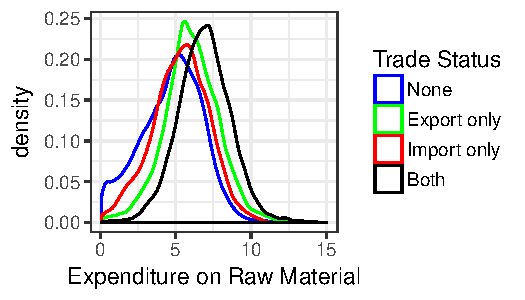
\includegraphics{./PICS/denslrawmat.pdf}   \\ 
 \input{./TABLES/sumstatslrawmat.gen}  \\  
\end{tabular}
\end{center}
\end{table}
\end{center}
\begin{center}
\begin{table}[H]
\begin{center}
\caption{Summary Statistics of Expenditure on Power and Fuel (log)}
\label{tab:lfuel}
\begin{tabular}{c}
 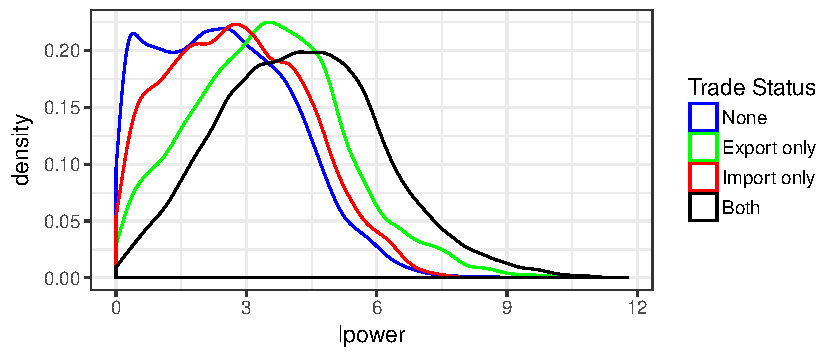
\includegraphics{./PICS/denslpower.pdf}   \\ 
 \input{./TABLES/sumstatslpower.gen}  \\  
\end{tabular}
\end{center}
\end{table}
\end{center}
\restoregeometry

\subsection{Appendix (Productivity Estimation OP)}\label{prodest}
\label{op}

 \textcite{olley1992dynamics} (OP) use the
following strategy to estimate the Cobb-Douglas function: 


The log transformation of the production function is written as : 
\begin{equation}
y_{it} = \beta_{o} + \beta_{l}l_{it} + \beta_{k}k_{it} + \omega_{it} + \epsilon_{it} 
\end{equation}
where $l_{it}$ is labour, $k_{it}$ is capital, $m_{it}$  is
the demand for materials, $\omega_{it}$ is firm-level-productivity
observable to the firm and $\epsilon_{it}$ are shocks to production.\\
The optimal investment decision of the firm is characterised by the following
function:
\begin{equation}
i_{it}= f_{k}(l_{it-1}, k_{it}, \omega_{it})
\end{equation}
The optimal labor decision is characterised by the following function:
\begin{equation}
l_{it}= f_{k}(l_{it-1}, k_{it}, \omega_{it})
\end{equation}

These are the assumptions made by \textbf{OP}:
\begin{enumerate}
\item $f_{k}(l_{it-1}, k_{it}, \omega_{it})$ is invertible in
  $\omega_{it}$
\item $\omega_{it}$ follows a first order markov process 
\item Investment at period i is not active until period $t+1$:
  $k_{it+1}= (1-\delta)k_{it} + i_{it}$
\item Labor is a perfectly flexible input i.e there are no labor
  adjustment cost
\end{enumerate}

The estimation procedure proceeds in two step:
\begin{enumerate}
\item Estimation of $\beta_{k}$:
Since $\omega_{it}=f_{k}^{-1}(l_{it-1},k_{it},i_{it})$ and inserting
this in the Cobb-Douglas equation to get: 
$$ y_{it} = \beta_{l}l_{it} + \phi_{it}(l_{it-1},i_{it},k_{it})$$
where $\phi_{it}(l_{it-1},i_{it},k_{it}) =  \beta_{k}k_{it}+ f_{k}^{-1}(l_{it-1},k_{it},i_{it})$
$\phi_{it}(l_{it-1},i_{it},k_{it})$ is approximated using a polynomial
expression and $beta_{l}$ is estimated by  OLS on the previous
equation
\item Estimation of $\beta_{k}$:
Since $\omega_{it}$ follows a first order markov process, it can be
written as: 
$$ \omega_{it} = h(\omega_{it-1}) + e_{it}$$
Then $\phi_{it}$ can be written as: 
$$ \phi_{it} = \beta_{k}k_{it} + h(\omega_{it-1}) + e_{it}$$
$$ \phi_{it} = \beta_{k}k_{it} + h(\phi_{it-1}- \beta_{k}k_{it-1}) + e_{it}$$
The unknown form of function h is approximated by quadratic function
and for any value of $\beta_k$ to get:
$$ \hat{\phi_{it}} = \beta_{k}k_{it} +\gamma_{0}
\gamma_{1}\hat{\omega_{it-1}^{\beta_{k}}}+
\gamma_{2}(\hat{\omega_{it-1}^{\beta_{k}}})^{2}
+ \gamma_{3}(\hat{\omega_{it-1}^{\beta_{k}}})^{3} $$
 This expression is minimised to get the estimate of $\beta_{k}$. 
\end{enumerate}
% \subsubsection{\textcite{levinsohn2003estimating} (LP)}

% \subsubsection{\textcite{ackerberg2006structural}(ACF)}
\newpage
\newgeometry{top=3cm}
\subsection{Appendix (Learning-by-doing)}\label{apendix:lbd}

\input{./TABLES/regLPcont.gen}
\input{./TABLES/prodcont.gen} 
\restoregeometry
\input{./TABLES/regACFcont.gen}
\input{./TABLES/prodACFcont.gen} 


\subsection{Appendix (Dynamic Random Effects Probit  Model)}\label{apendix:random}
Let i be the unit and t be the time. A dynamic random effects probit
is written as: 
$$ y_{it}^{*} = \gamma y_{i,t-1} + x_{it}'\beta + \alpha_{i} +
\epsilon_{it}; y_{it}=1[y_{it}^{*} > 0]$$
where $\gamma$ is the state dependence parameter.



There are three ways to estimate the above equation: 
\begin{enumerate}
\item Treat $y_{i1}$ as exogenously given and do not explain it
\item Heckman Method
\item Wooldridge Method
\end{enumerate} 
I use the Wooldridge method which assumes that $\alpha_{i}$:
$$\alpha_{i} = \lambda y_{i1} + \tilde{\alpha_{i}}$$

Assumptions: 

\begin{enumerate}
\item The i-units are a random sample
\item $\epsilon_{it} \sim N(0,1)$ is independent of $x_{i}$
\item $\tilde{\alpha_{i}} \sim N(0,\sigma_{alpha}^{2})$ is independent of
  $x_{i}$ and $\epsilon_{it}$
\end{enumerate}

The likelihood function is given by:
$$ L_{i}(\beta, \gamma, \sigma_{\alpha},\lambda)= \int_{-\infty}^{\infty}
\prod_{t=2}^{T}\Phi(x^{'}_{it}\beta + \gamma y_{it-1} + \lambda y_{i1} +
\tilde{\alpha}) \frac{\phi(\tilde{\alpha})}{\sigma_{\tilde{\alpha}}}
d\tilde{\alpha}$$ 

$$ L(\beta, \gamma, \sigma_{\alpha},\lambda) = \prod_{i=1}^{N}L_{i}(\beta, \gamma, \sigma_{\alpha},\lambda:y_{i},x_{i}$$
The marginal effects are given by:
\begin{equation}
\frac{\delta E[y_{it}|x_{it}, \alpha_{i}]}{\delta x_{it,j}} =
\beta_{j}\phi(x_{it}^{'} \beta + \alpha_{i})
\end{equation}

I report the average marginal effects which are given by: 
$$ \frac{1}{N} \sum_{i}\phi( x_{it}^{'} \beta + \alpha_{i})
\hat{\beta_{j}}$$

\newgeometry{top=4cm}
\begin{center}
\begin{table}[H]
\caption{Dynamic Random Effects Probit (ACF Estimates)}
\label{tab:dynprobitacf}
\begin{center}
\begin{tabular}{l*{4}{c}}
\hline\hline&\multicolumn{2}{c}{Export
              Decision}&\multicolumn{2}{c}{Import Decision}\\
            &\multicolumn{1}{c}{(1)}&\multicolumn{1}{c}{(2)}&\multicolumn{1}{c}{(3)}&\multicolumn{1}{c}{(4)}\\
            &\multicolumn{1}{c}{Base}&\multicolumn{1}{c}{Lagged}&\multicolumn{1}{c}{Base}&\multicolumn{1}{c}{Lagged}\\
&\multicolumn{1}{c}{}&\multicolumn{1}{c}{Complementarity}&\multicolumn{1}{c}{}&\multicolumn{1}{c}{Complementarity}\\
\hline
main        &                     &                     &                     &                     \\
$d_{it-1}^{X}$      &       1.834$^{***}$&       1.786$^{***}$&                     &       0.380$^{***}$\\
                   &      (71.18)         &     (68.65)          &     (16.31)         &\\
[1em]                
$d_{it-1}^{M}$                            &       0.370$^{***}$&       1.600$^{***}$&       1.554$^{***}$\\
            &                             &     (14.67)         &     (66.32)         &     (63.85)         \\
[1em]                
$\hat{\omega}_{it}$ &       0.216$^{***}$&       0.198$^{***}$&       0.277$^{***}$&       0.266$^{***}$\\
                    &     (15.83)         &     (14.70)         &     (21.51)         &     (21.16)         \\
[1em]                
$k_{it}$            &      0.0748$^{***}$&      0.0539$^{***}$&       0.119$^{***}$&       0.110$^{***}$\\
            &              (5.74)         &      (4.19)         &      (9.75)         &      (9.27)         \\
[1em]                
$l_{it}$     &              0.226$^{***}$&       0.201$^{***}$&       0.234$^{***}$&       0.206$^{***}$\\
                    &     (16.48)         &     (14.80)         &     (18.91)         &     (16.99)         \\
[1em]                
$d_{i1}^{X}$          &      1.333$^{***}$&       1.264$^{***}$&                     &                     \\
                    &     (29.35)         &     (28.62)         &                     &                     \\
[1em]                
$d_{i1}^{M}$          &                    &                     &       1.081$^{***}$&       0.986$^{***}$\\
                    &                     &                     &     (28.27)         &     (26.62)         \\
[1em]                
\_cons              &      -3.264$^{***}$&      -3.122$^{***}$&      -3.655$^{***}$&      -3.617$^{***}$\\
                    &    (-25.05)         &    (-24.47)         &    (-28.64)         &    (-29.17)         \\
rho                 &     (-7.15)         &     (-8.36)         &    (-10.65)         &    (-12.25)         \\
$\sigma^{2}_{\alpha}$   &    0.392         &       0.373         &       0.348         &       0.321         \\
                     &       0.804         &       0.771         &       0.731&       0.687         \\
                    &  (0.025) & (0.023)& (0.021)& (0.021) \\
Log-Likelihood      &    -14513.0         &    -14406.6         &    -15879.7         &    -15749.5         \\
\hline\hline
Industry Dummies & Yes& Yes& Yes& Yes\\
Time Dummies& Yes& Yes& Yes& Yes\\
\hline\hline
\multicolumn{5}{l}{\footnotesize \textit{t} statistics in parentheses}\\
\multicolumn{5}{l}{\footnotesize $^{*}$ \(p<0.05\), $^{**}$ \(p<0.01\), $^{***}$ \(p<0.001\)}\\
\end{tabular}
\end{center}
\end{table}
\end{center}
\restoregeometry
\subsection{Appendix (Dynamic Bivariate Probit Model)}\label{apendix:bivariate}
Let the latent model be: 
$$y^{1*}_{it}= x_{it}^{T}\beta_{1} + y_{it-1}\gamma + \varepsilon_{it}^{1}$$
$$y^{2*}_{it}= x_{it}^{T}\beta_{2} +y_{1t-1}\gamma + \varepsilon_{it}^{2}$$

we have the observed responses as, 
$$y_{it}^{1}= I(y^{1*}_{it}>0)$$
$$y_{it}^{2}= I(y^{2*}_{it}>0)$$

The error distribution is given as follows,
$$(\varepsilon_{it}^{1}, \varepsilon_{it}^{2}) \sim N \begin{pmatrix} 0, & \begin{pmatrix}1 & \rho\\ \rho & 1\end{pmatrix} 
\end{pmatrix}$$

The multivariate normal density  of $f(y^{1*}_{it}, y^{2*}_{it})$  given the assumption above is given by: 
\begin{equation}
\begin{aligned}
    f(y_{it}^{1},y_{it}^{2}) = \frac{1}{2\pi \sigma_{y_{it}^{1}}\sigma_{y_{it}^{2}}\sqrt{1-\rho^2}} exp(\frac{-1}{2(1-\rho^2)} [\frac{(y_{it}^{1} - \mu_{y_{it}^{1}})^2}{\sigma_{y_{it}^{1}}^{2}} + \\
    \frac{(y_{it}^{2} - \mu_{y_{it}^{2}})^2}{\sigma_{y_{it}^{2}}^{2}} 
    -2 \rho \frac{(y_{it}^{1} - \mu_{y_{it}^{1}}) (y_{it}^{2} - \mu_{y_{it}^{2}})
    }{\sigma_{y_{it}^{1}}\sigma_{y_{it}^{2}}}]
  \end{aligned}
\end{equation}
Therefore the likelihood function is given by 

\begin{equation}
\begin{aligned}
L(\beta_1,\beta_2,\gamma_1,\gamma_2) = \Big( \prod
P(Y_{it}^{1}=1,Y_{it}^{2}=1\mid\beta_1,\beta_2,\gamma_1,\gamma_2)^{Y_{it}^{1}Y_{it}^{2}}\\
 P(Y_{it}^{1}=0,Y_{it}^{2}=1\mid\beta_1,\beta_2,\gamma_1,\gamma_2)^{(1-Y_{it}^{1})Y_{it}^{2}}  \\
P(Y_{it}^{1}=1,Y_{it}^{2}=0\mid\beta_1,\beta_2,\gamma_1,\gamma_2)^{Y_{it}^{1}(1-Y_{it}^{2})}\\
P(Y_{it}^{1}=0,Y_{it}^{2}=0\mid\beta_1,\beta_2,\gamma_1,\gamma_2)^{(1-Y_{it}^{1})(1-Y_{it}^{2})} \Big)
\end{aligned}
\end{equation}




% \begin{equation}
% \begin{aligned}
% L(\beta_1,\beta_2) = \sum(\Phi( Y_{1i,t}Y_{2i,t}\ln \Phi(X_1\beta_1,X_2\beta_2,\rho) \\
%  + (1-Y_{1i,t})Y_{2i,t}\ln \Phi(-X_1\beta_1,X_2\beta_2,-\rho) \\
% + Y_{1i,t}(1-Y_{2i,t})\ln \Phi(X_1\beta_1,-X_2\beta_2,-\rho) \\
%  +(1-Y_{1i,t})(1-Y_{2i,t})\ln \Phi(-X_1\beta_1,-X_2\beta_2,\rho) \Big))\\
% \end{aligned}
% \end{equation}
\begin{center}
\begin{table}[H]
\caption{Dynamic Bivariate Probit (ACF Estimates)}
\label{tab:biprobitacf}
\begin{center}
\begin{tabular}{l*{2}{c}}
\hline\hline
            &\multicolumn{1}{c}{(1)}&\multicolumn{1}{c}{(2)}\\
            &\multicolumn{1}{c}{Export
              Decsion}&\multicolumn{1}{c}{Import Decision}\\
\hline\\
$d_{it-1}^{X}$   &       2.539$^{***}$   &       0.397$^{***}$\\
            &        (0.0312)            &    (0.0273)         \\
[1em]                                                          
$d_{it-1}^{M}$   &       0.360$^{***}$   &       2.175$^{***}$\\
            &        (0.0278)            &    (0.0335)         \\
[1em]                                                          
$\hat{\omega}_{it}$&       0.103$^{***}$   &       0.165$^{***}$\\
            &        (0.0152)            &    (0.0150)         \\
[1em]                                                          
$k_{it}$       &       0.0125            &      0.0848$^{***}$\\
            &        (0.0157)            &    (0.0123)         \\
[1em]                                                          
$l_{it}$     &          0.143$^{***}$   &       0.146$^{***}$\\
            &        (0.0173)            &    (0.0173)         \\
[1em]                                                          
Constant      &        -2.212$^{***}$   &      -2.768$^{***}$\\
            &         (0.111)            &    (0.0809)         \\
\hline
\hline
      &                     \\
$\rho$      &       0.439$^{***}$\\
            &    (0.0173)         \\
LR test& $\rho=0$, $\chi^{2}(1)= 641.78$&\\
& p=0.000&\\
Industry Dummies & Yes& \\
Time Dummies& Yes& \\
\hline\hline
\multicolumn{2}{r}{\footnotesize Standard errors in parentheses}\\
\multicolumn{2}{r}{\footnotesize $^{*}$ \(p<0.05\), $^{**}$ \(p<0.01\), $^{***}$ \(p<0.001\)}\\
\end{tabular}
\end{center}

\end{table}
\end{center} 


\end{document}
